\section{Технологическая часть}
	\subsection{Средства реализации программного обеспечения}
		\subsubsection{Язык программирования}
			При разработке программного продукта был использован язык программирования Python (версия 3.7.2) \cite{python}.
			
			Данный выбор был сделан по следующим причинам.
			\begin{enumerate}
				\item[1)] Опыт работы с рассматриваемым языком.
				\item[2)] Поддержка ООП.
				\item[3)] Большое количество литературы, связанной с ЯП Python.
				\item[4)] Широкая применимость.
			\end{enumerate}
		
			В качестве среды разработки были использованы PyCharm \cite{pycharm} и Visual Studio Code \cite{vcode}, поскольку они бесплатны для студентов, удобны в процессе разработки и ранее активно использовались.

		\subsubsection{СУБД}
		Одними из наиболее популярных СУБД, используемых в настоящее время, являются Oracle, MySQL, Microsotf SQL сервер и PostgreSQL. В таблице \ref{cmptable} приведено их сравнение.
		
		\begin{table}[pt!] 
			\begin{center}
				\caption{Сравнение СУБД}
				\label{cmptable}
				\begin{tabular}{| p{4cm} | p{5cm} | p{5cm} |}
					\hline
					\textbf{СУБД} 	& \textbf{Преимущества} & \textbf{Недостатки} \\
					\hline
					Oracle 			& - Широкий функционал & - Платное использование \\ 
									& - Ориентирован на работу с большими БД & - Необходимость в дополнительных ресурсах \\
					\hline
					MySQL 			& - Есть бесплатная версия & - Есть платные версии для коммерческого использования\\
									& - Исчерпывающая документация & - Для бесплатной версии доступна только платная поддержка \\ 
									& - Простой интерфейс & - Отсутствует встроенная поддержка XML \\
									& - Хорошо справляется с большими объёмами данных &  \\
					\hline
					Microsotf SQL сервер  	& - Низкий порог вхождения &- Высокая цена для юридических лиц \\
					 				& - Стабильность в работе & - Требуется много дополнительных ресурсов \\ 
									& - Возможность регулировать и отслеживать уровень производительности &  \\
					\hline
					PostgreSQL 		& - Бесплатная & - Низкая скорость выполнения пакетных операций \\ 
									& - Подробная документация & - Поддерживается не всеми библиотеками \\
									& - Поддержка json &  \\
					\hline
				\end{tabular}
			\end{center}
		\end{table}
	\newpage
	
	Поскольку есть опыт работы с такой СУБД, как PostgreSQL \cite{postgresql}, то это средство было выбрано для реализации текущей задачи.
	
	Что касается ORM (Object-relational mapping), то был выбран peewee \cite{peewee}, поскольку также хорошо знаком, так как активно использовался ранее.
	
	\subsubsection{Web-фреймворк}
	Django \cite{django} был выбран в качестве Web-фреймворка по следующим причинам.
	\begin{itemize}
		\item Использует шаблон проектирования MVC, который был выбран ранее.
		\item Работает с большим количеством дополнительных функций, которые значительно упрощают работу с аутентификацией пользователя, картами сайта и т.д.
		\item Масштабируемость.
	\end{itemize}

	\subsection{UML-диаграммы}
		\subsubsection{Компонент доступа к данным}
		Доступ к данным реализован с помощью паттерна проектирования Repository. Соответствующая UML-диаграмма представлена на рисунке \ref{fig6:image}.
		
		\begin{figure}[ph!]
			\centering
			\begin{center}
				{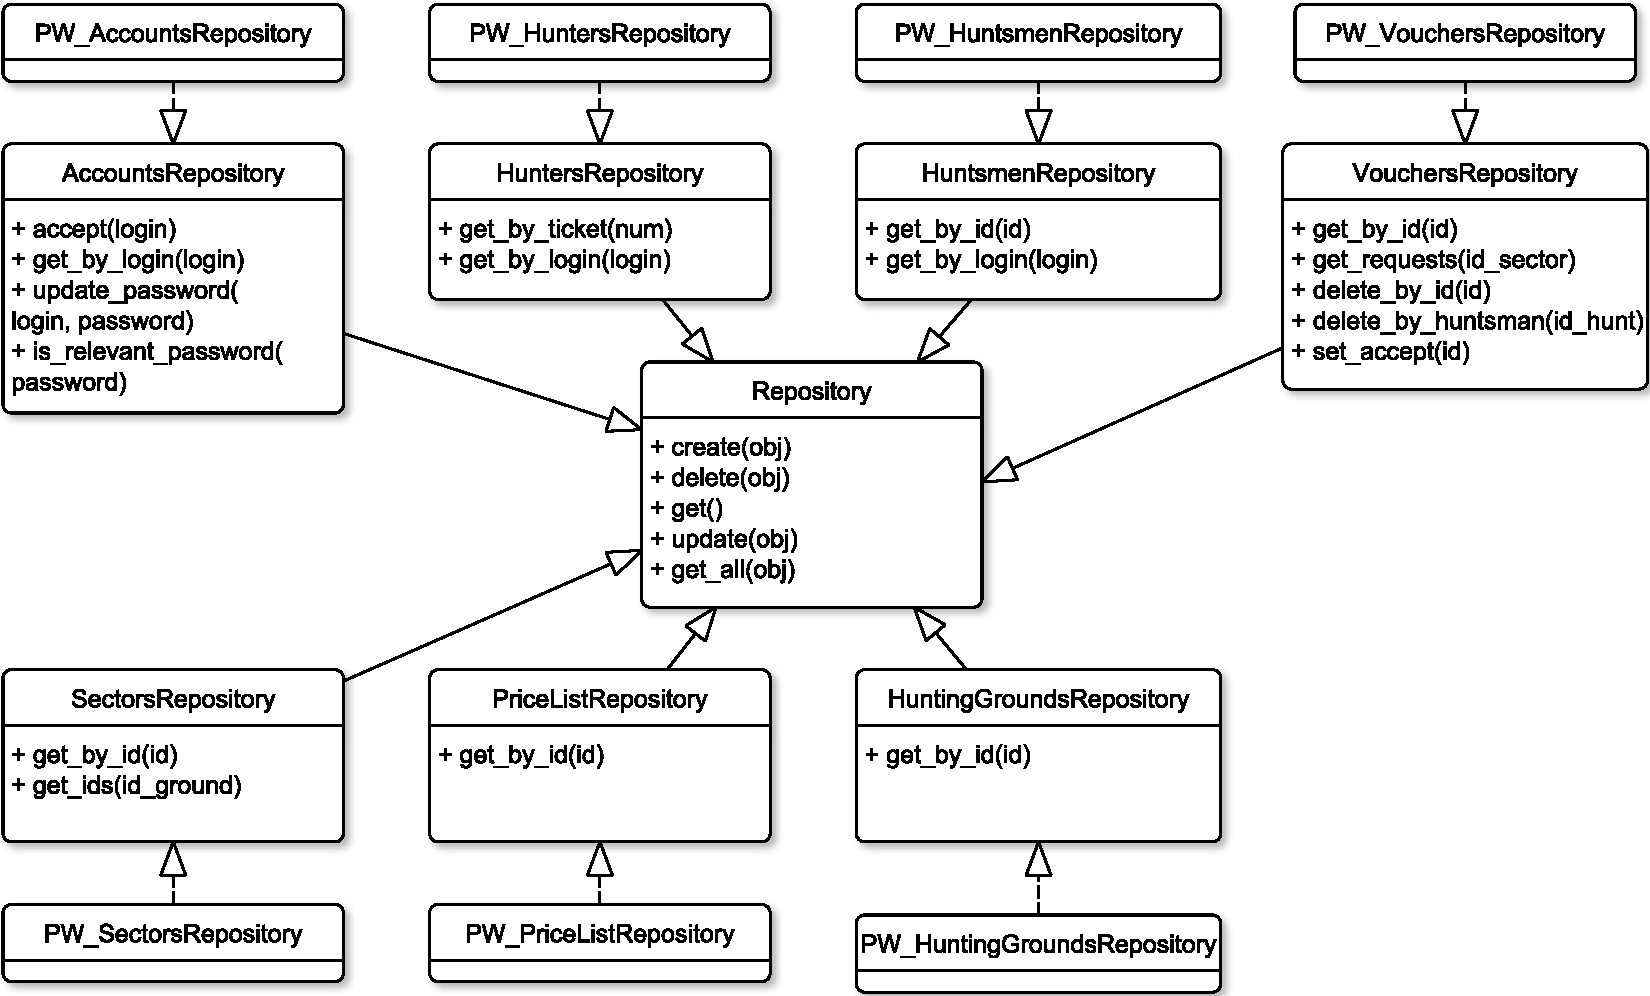
\includegraphics[scale=0.6]{schemes/uml_access_rep.pdf}}
				\caption{UML-диаграмма компонента доступа к данным}
				\label{fig6:image}
			\end{center}
		\end{figure}
		\newpage
	
		\subsubsection{Компонент бизнес-логики}
		Этот компонент выполняет основную обработку данных, соответствующая UML-диаграмма представлена на рисунке \ref{fig7:image}.
		
		\begin{figure}[ph!]
			\centering
			\begin{center}
				{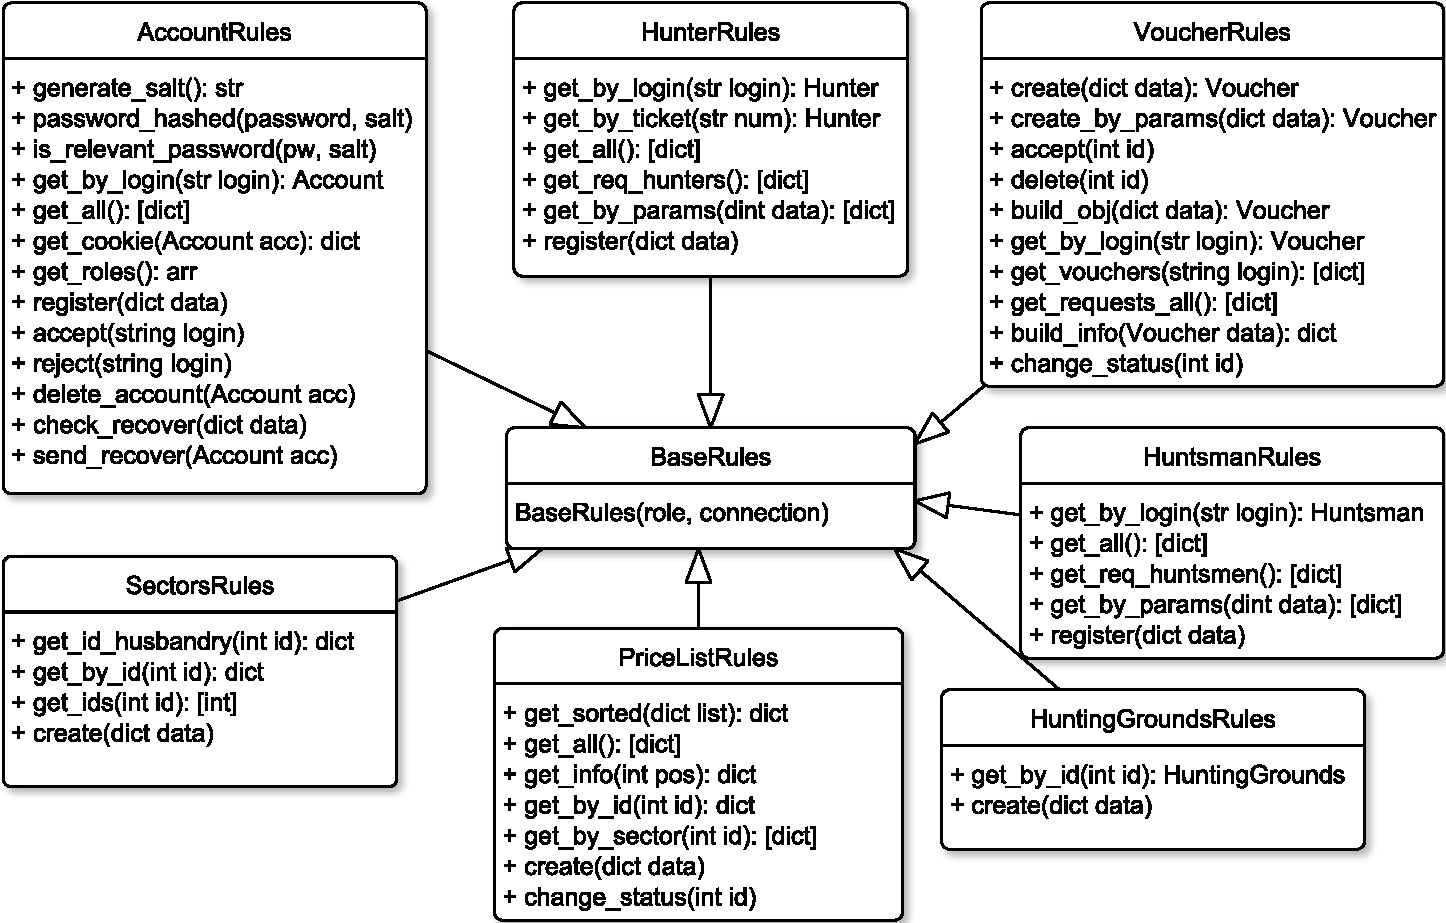
\includegraphics[scale=0.6]{schemes/uml_business.pdf}}
				\caption{UML-диаграмма компонента бизнес-логики}
				\label{fig7:image}
			\end{center}
		\end{figure}
	
		\subsubsection{Компонент представления}
		UML-диаграмма компонента, отвечающего за отображение web-страниц, изображена на рисунке \ref{fig8:image}.
		
		\begin{figure}[pt!]
			\centering
			\begin{center}
				{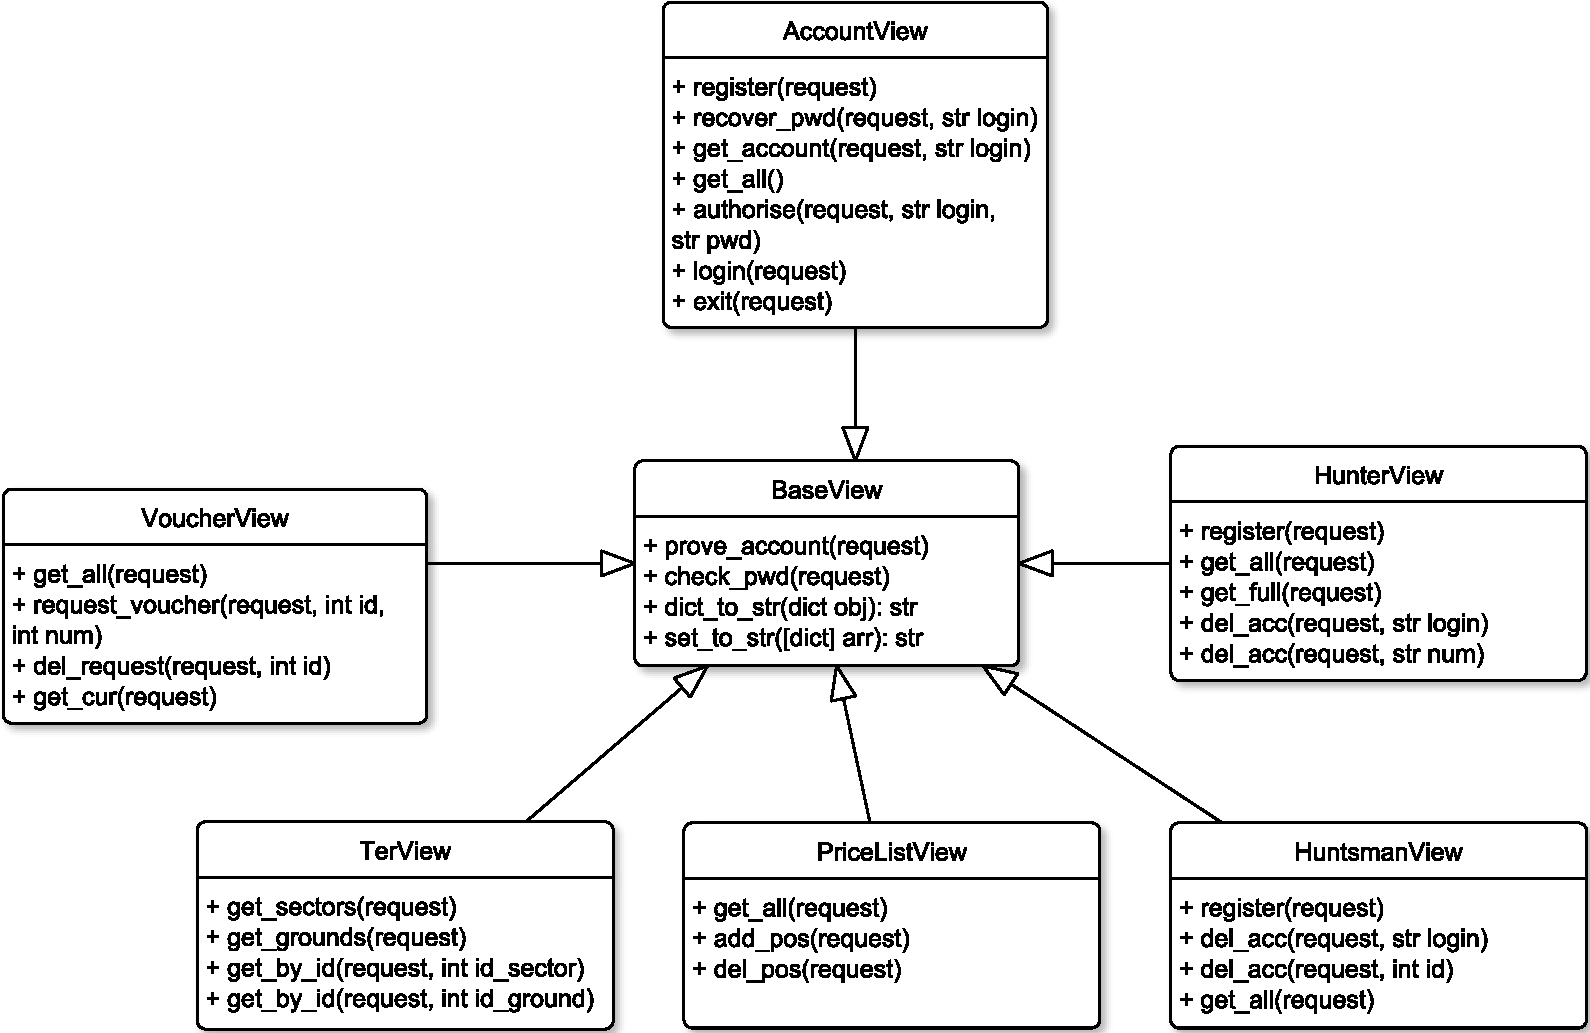
\includegraphics[scale=0.6]{schemes/webGUI.pdf}}
				\caption{UML-диаграмма компонента бизнес-логики}
				\label{fig8:image}
			\end{center}
		\end{figure}
		\newpage
	
		\subsubsection{Диаграмма приложения}
		Все приведённые выше UML-диаграммы \ref{fig6:image}-\ref{fig8:image} можно объединить в одну - диаграмму-приложения, которая находится на рисунке \ref{fig9:image}.
		
		\begin{figure}[ph!]
			\centering
			\begin{center}
				{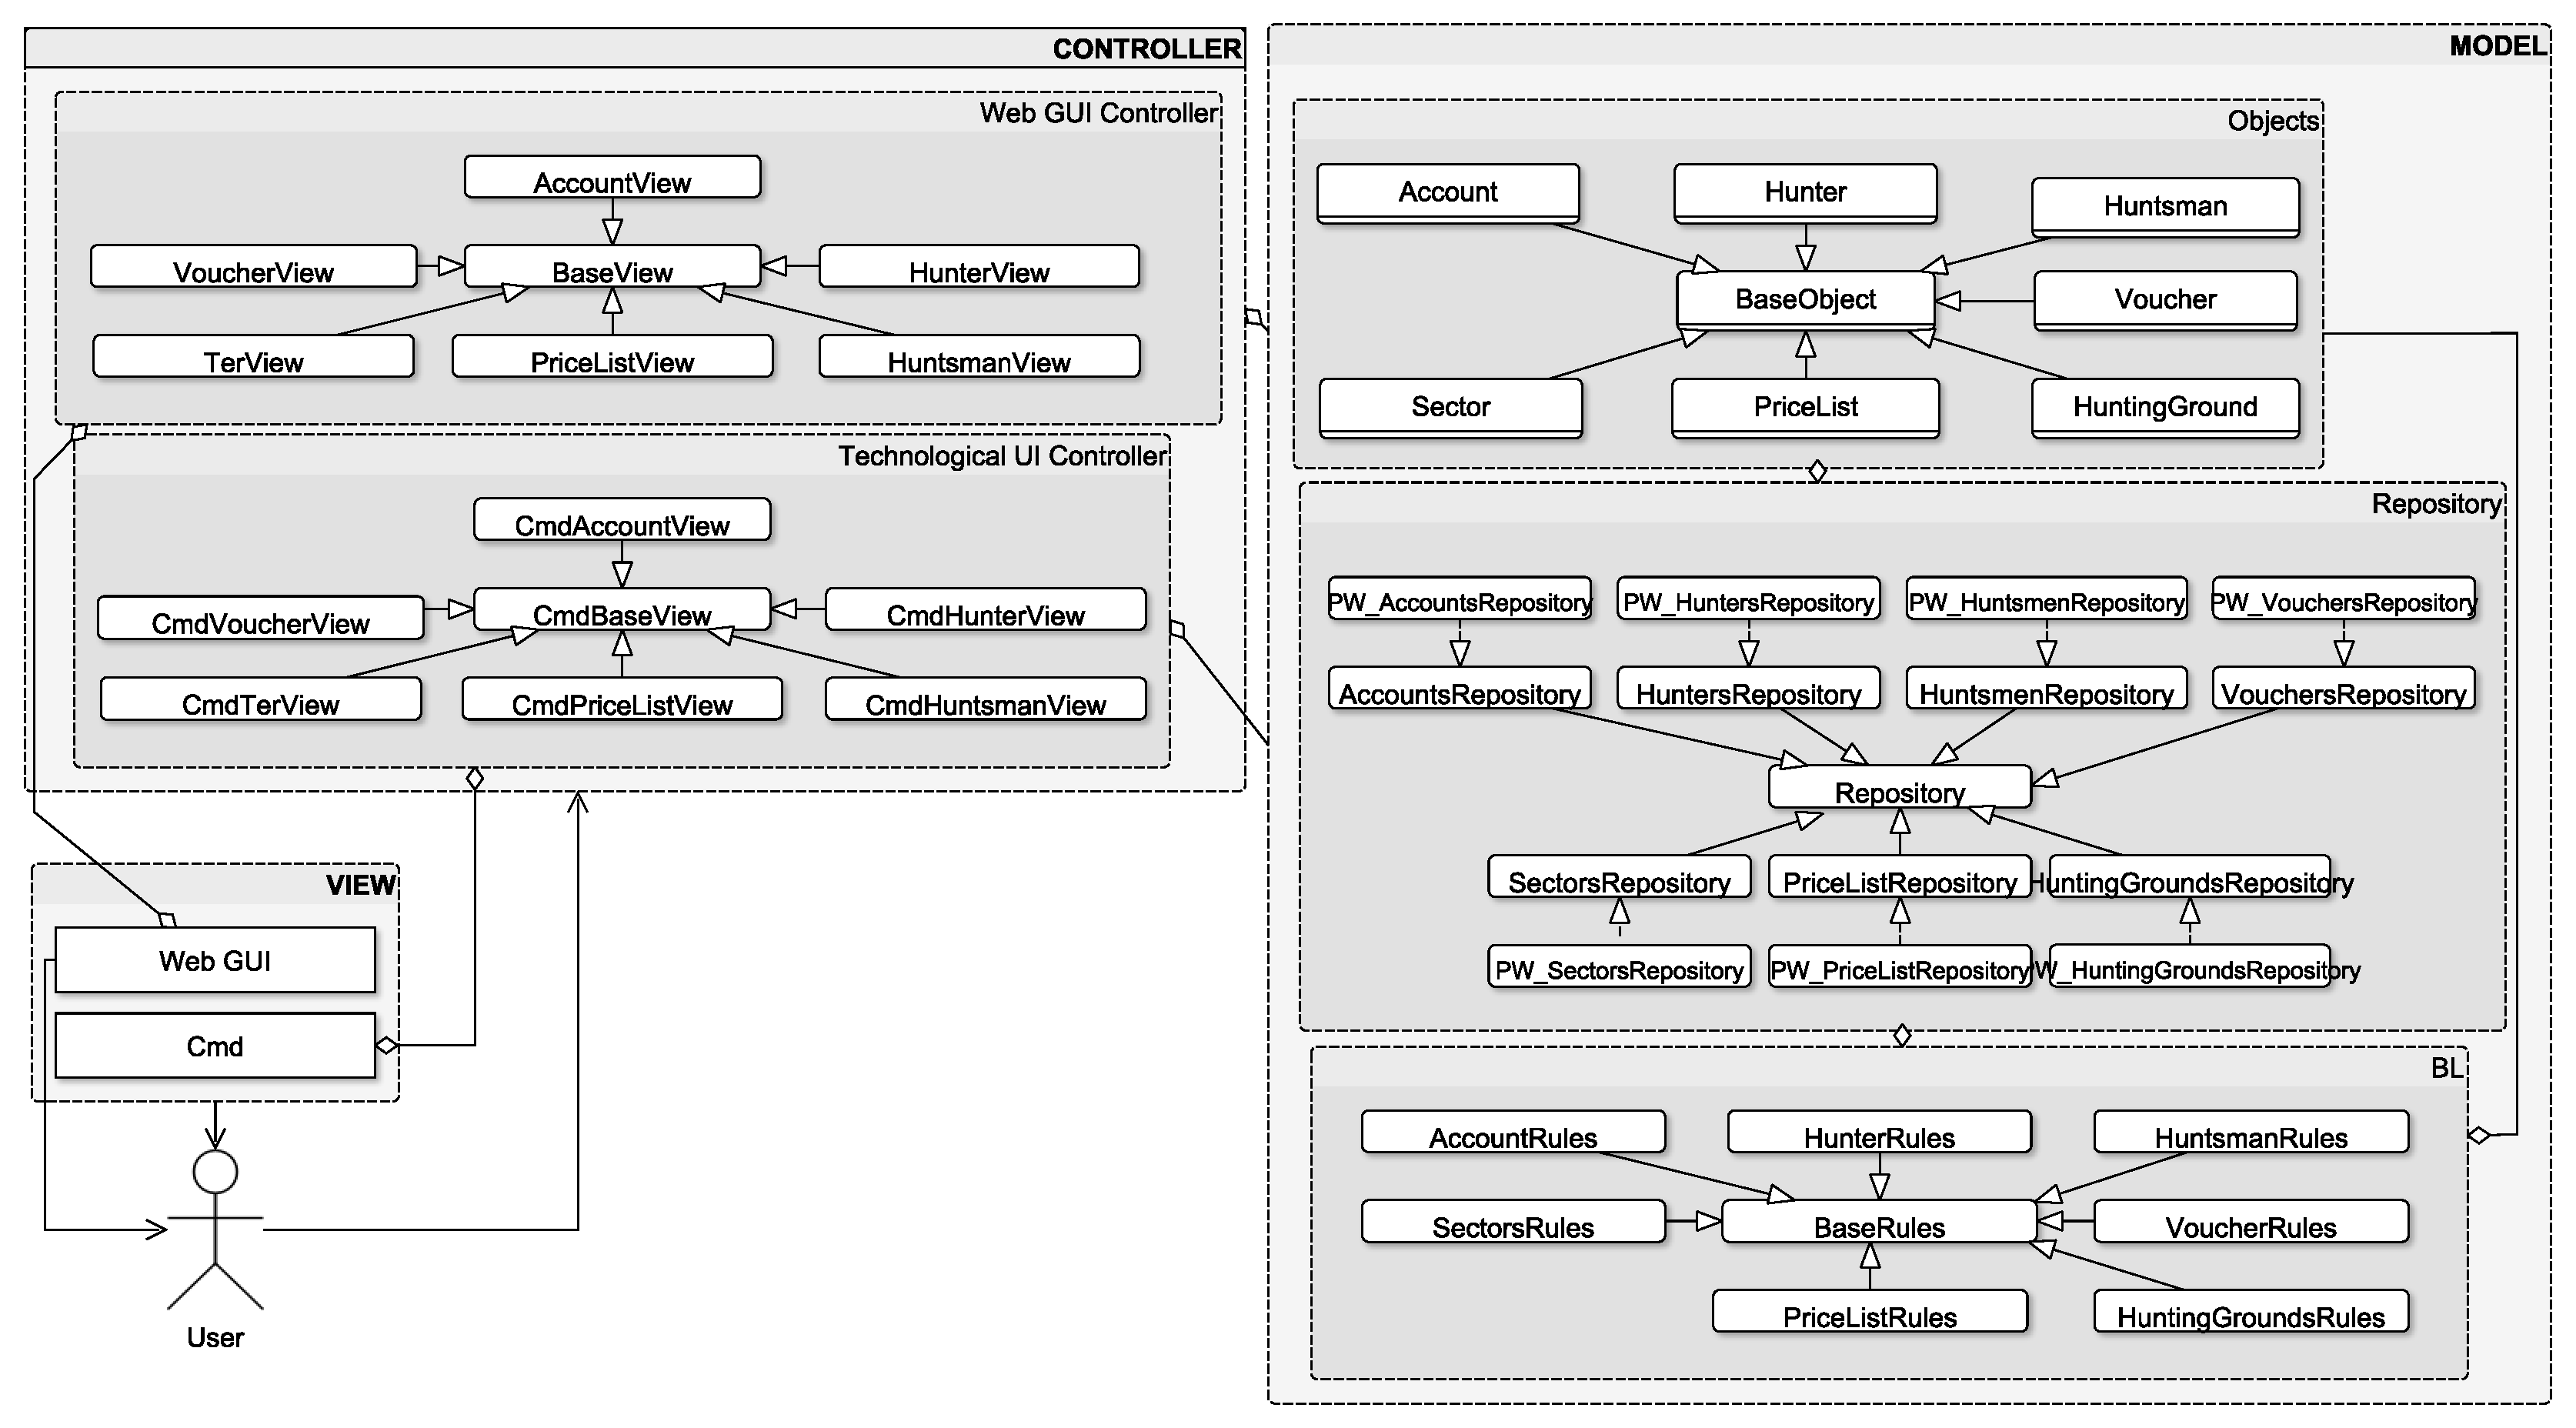
\includegraphics[scale=0.44, angle=90]{schemes/uml_full.pdf}}
				\caption{UML-диаграмма компонента бизнес-логики}
				\label{fig9:image}
			\end{center}
		\end{figure}
	\newpage
	
	\subsection{Реализация базы данных}	
		\subsubsection{Создание таблиц}
		В соответствии с моделью были созданы 7 таблиц. Создание некоторых из них, а именно accounts, hunters, huntsmen представлено в листинге \ref{lst:create_tables}.
		
		\begin{lstlisting}[caption = {Создание некоторых таблиц}, label=lst:create_tables]
CREATE TABLE IF NOT EXISTS accounts(
	login VARCHAR(20) PRIMARY KEY,
	salt TEXT,
	hashed_password TEXT,
	surname VARCHAR(30) NOT NULL,
	firstname VARCHAR(30) NOT NULL,
	patronymic VARCHAR(30),
	date_of_birth DATE NOT NULL,
	sex CHAR NOT NULL,
	mobile_phone VARCHAR(30) NOT NULL,
	email VARCHAR(50) NOT NULL,
	type_role VARCHAR(10) NOT NULL
);

CREATE TABLE IF NOT EXISTS huntsmen(
	id INTEGER REFERENCES sectors,
	PRIMARY KEY (id),
	login VARCHAR(20) REFERENCES accounts
);

CREATE TABLE IF NOT EXISTS hunters(
	ticket_num TEXT PRIMARY KEY,
	residence VARCHAR(100) NOT NULL,
	login VARCHAR(20) REFERENCES accounts
);
		\end{lstlisting}
	
		В таблице accounts первичный ключ - login (логин пользователя), атрибуты surname, firstname, patronymic, mobile\_phone, email, type\_role имеют органичения в несколько символов, также дата рождения имеет специальный тип - дата. В основном, на все поля выставлено ограничение NOT NULL, поскольку эти поля обязательны и заполняются пользователем (это не касается отчества, поскольку его может не быть). Касаемо двух других таблиц, то у них выставлены такие же ограничения.
		
		В таблице huntsmen первичный ключ - id (идентификатор сектора, за которым он закреплён), он же и внешний ключ, который ссылается на одноимённое поле в таблице sectors, также внешним ключом является атрибут login, указывающий на соответствующее поле в таблице accounts.
		
		ticket\_num (номер охотничьего билета) - первичный ключ в таблице hunters, а login также как и в таблице huntsmen выступает в качестве внешнего ключа на таблицу accounts.
			
		\subsubsection{Наполнение таблиц}
		Таблицы заполняются сгенерированными данными с помощью библиотеки Faker. Полученные данные записываются в файл, из которого далее будут подгружаться данные. На листингах \ref{lst:create_faker1}-\ref{lst:create_faker2} приведены функции генерации данных для таблицы аккаунтов (accounts) и путёвок (vouchers), примеры таких функций.
		
		\begin{lstlisting}[caption = {Генерация данных для таблицы accounts}, label=lst:create_faker1]
def generate_accounts():
	fake = Faker()
	fake_ru = Faker('ru_Ru')
	
	f = open('accounts.cvg', 'w')
	
	i = 0
	while i < NUM_SECTORS + MAX_AMOUNT:
		sex_p = choice(sex)
		if sex_p == 'м':
			surname = fake_ru.last_name_male()
			name = fake_ru.first_name_male()
			patronymic = fake_ru.middle_name_male()
		else:
			surname = fake_ru.last_name_female()
			name = fake_ru.first_name_female()
			patronymic = fake_ru.middle_name_female()
		
		date_of_brth = fake_ru.date_of_birth(None, 21, 80)
		phone = fake_ru.phone_number()
		email = fake_ru.email()
		
		lgn = surname[:3] + name[:2] + '_' + str(date_of_brth).split('-')[2] + \
		'_' + str(date_of_brth).split('-')[1] + \
		'_' + str(date_of_brth).split('-')[0]
		lgn = pytils.translit.translify(lgn)
		login.append(lgn)
		
		pswd = fake.password(length=8, special_chars=False, digits=True, upper_case=True, lower_case=True)
		salt = uuid.uuid4().hex
		salt_pw = pswd.encode('utf-8') + salt.encode('utf-8')
		hashed_pswd = hashlib.sha256(salt_pw).hexdigest()
		
		if i < NUM_SECTORS:	status = 'егерь'
		else:				status = 'охотник'
		
		line = "{0}|{1}|{2}|{3}|{4}|{5}|{6}|{7}|{8}|{9}|{10}\n".format(
			lgn, salt, hashed_pswd, surname, name,
			patronymic, date_of_brth, sex_p, phone, email, status)
		f.write(line)
		
		i += 1
	
	f.close()
		\end{lstlisting}
	
	\begin{lstlisting}[caption = {Генерация данных для таблицы vouchers}, label=lst:create_faker2]
def generate_vouchers():
	f = open('vouchers.cvg', 'w')
	
	for i in range(MAX_AMOUNT + 200):
		duration = choice(range(1, 100))
		amount = choice(range(1, 10))
		prc = 0
		ind = choice(range(1, MAX_AMOUNT))
		id_hunter = hunters[ind]
		id_pricelist = choice(range(1, MAX_AMOUNT))
		
		line = "{0}|{1}|{2}|{3}|{4}\n".format(duration, amount, prc, id_hunter, id_pricelist)
		
		f.write(line)
	f.close()
	\end{lstlisting}
		
		
		\subsubsection{Реализация триггеров}
		\subsubsection{Реализация ролевой модели}
		Для того, чтобы предоставить необходимые права доступа разным категориям пользователей (admin, huntsman, hunter), была реализована ролевая модель на уровне базы данных. Код, в котором они задаются, представлен в листингах \ref{lst:create_rights_admin}-\ref{lst:create_rights_hunter}. Другие таблицы заполняются аналогично.
		
		\begin{lstlisting}[caption = {Создание админа}, label=lst:create_rights_admin]
CREATE ROLE admin WITH
	LOGIN
	SUPERUSER
	CREATEDB
	CREATEROLE
	NOREPLICATION
	PASSWORD 'admin'
	CONNECTION LIMIT -1;
		\end{lstlisting}
	
		\begin{lstlisting}[caption = {Создание huntsman и задание прав}, label=lst:create_rights_huntsman]
CREATE ROLE huntsman WITH
	LOGIN
	NOSUPERUSER
	NOCREATEDB
	NOCREATEROLE
	NOREPLICATION
	PASSWORD 'huntsman'
	CONNECTION LIMIT -1;
	
GRANT SELECT ON price_list TO huntsman;
GRANT SELECT ON accounts TO huntsman;
GRANT SELECT ON huntsmen TO huntsman;
GRANT SELECT ON hunters TO huntsman;
GRANT SELECT ON sectors TO huntsman;
GRANT SELECT ON vouchers TO huntsman;
GRANT SELECT ON hunting_grounds TO huntsman;

GRANT UPDATE ON vouchers TO huntsman;

GRANT DELETE ON vouchers TO huntsman;
GRANT DELETE ON hunters TO huntsman;

GRANT INSERT ON vouchers TO huntsman;

GRANT ALL PRIVILEGES ON SEQUENCE vouchers_id_seq TO huntsman;
		\end{lstlisting}
	
		\begin{lstlisting}[caption = {Создание hunter и задание прав}, label=lst:create_rights_hunter]
CREATE ROLE hunter WITH
	LOGIN
	NOSUPERUSER
	NOCREATEDB
	NOCREATEROLE
	NOREPLICATION
	PASSWORD 'hunter'
	CONNECTION LIMIT -1;
	
GRANT SELECT ON price_list TO hunter;
GRANT SELECT ON accounts TO hunter;
GRANT SELECT ON sectors TO hunter;
GRANT SELECT ON hunting_grounds TO hunter;
GRANT SELECT ON hunters TO hunter;
GRANT SELECT ON vouchers TO hunter;
GRANT SELECT ON huntsmen TO hunter;

GRANT ALL PRIVILEGES ON SEQUENCE vouchers_id_seq TO hunter;

GRANT INSERT ON vouchers TO hunter;
GRANT INSERT VALUES('id', 'amount_animals', 'price', 'id_hunter', 'id_pricelist', 'status') INTO vouchers TO hunter;

GRANT DELETE ON vouchers TO hunter;
		\end{lstlisting}
		
	\subsection{Интерфейс приложения}
	Для визуальной демонстрации приложения рассмотрим страницы, которые задействуются при оформлении путёвки. Сделать это может как охотник, так и егерь с администратором. 
	
	
	Для всех пользователей переход между страницами приложения осуществляется путём выбора пункта из верхнего меню. Например, чтобы подать заявку на путёвку пользователь должен из верхнего меню (рисунок \ref{fig10:image}) навести мышкой на пункт <<ПУТЁВКИ>>, и затем, из выпадающего списка выбрать действие <<Купить>>.
	
	\begin{figure}[h]
		\centering
		\begin{center}
			{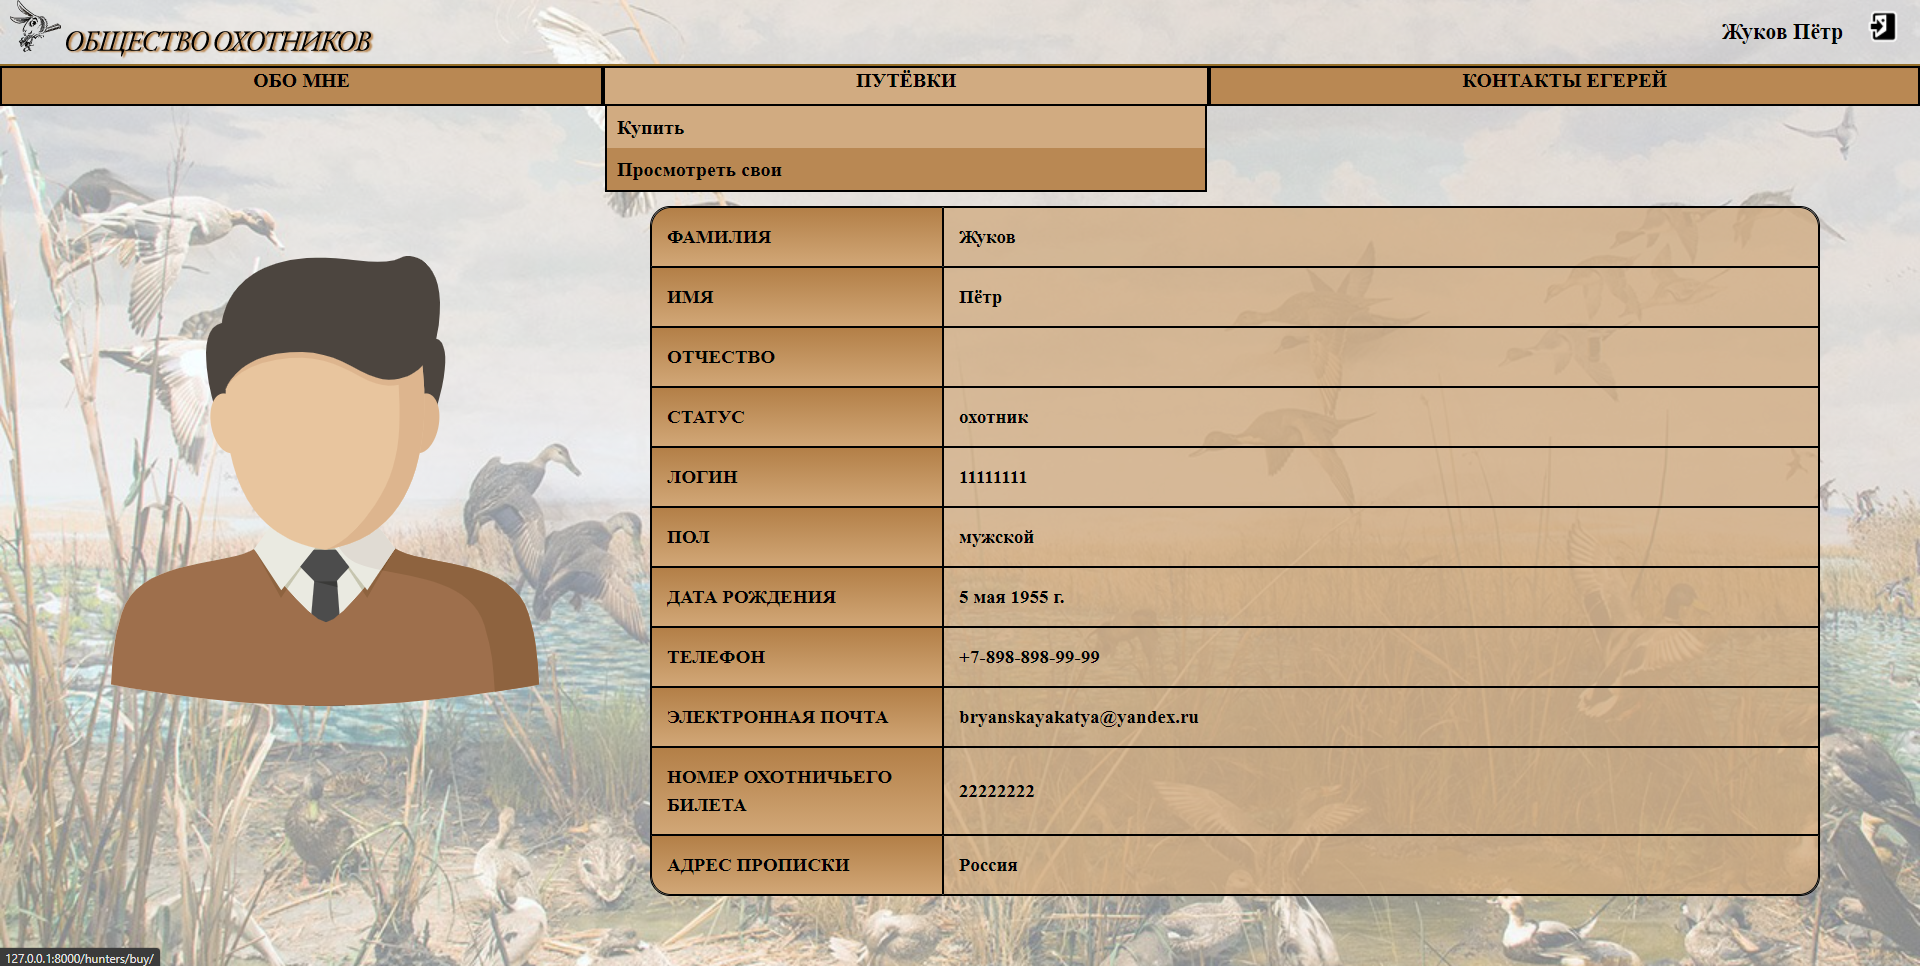
\includegraphics[scale=0.34]{schemes/screens/start.png}}
			\caption{Переход на страницу подачи заявки на путёвку}
			\label{fig10:image}
		\end{center}
	\end{figure}

	После этого охотник попадает на страницу, изображенную на рисунке \ref{fig11:image}. На ней приведён полный список всех доступных путёвок по всем хозяйствам и секторам. Используя мышь или правую полосу прокрутки можно ознакомиться со всем списком. 
	
	Каждая позиция из списка содержит информацию о месте (название хозяйства) и номере сектора, названии животного, на которого выдаётся разрешение, и цена за 1 единицу. 
	
	В поле <<Количество>> пользователь может указать, на сколько животных он хотел бы оформить путёвку. Для этого достаточно нажать кнопкой мыши на это поле в соответствующей строке из прайс-листа. Пользователь может указать число от 1 до 99, причём чтобы контролировать число отстреленных животных только егерь, закрепленный за данным сектором, или администратор может принимать решение одабривать такую заявку или, наоборот, отклонить. 
	
	\begin{figure}[h]
		\centering
		\begin{center}
			{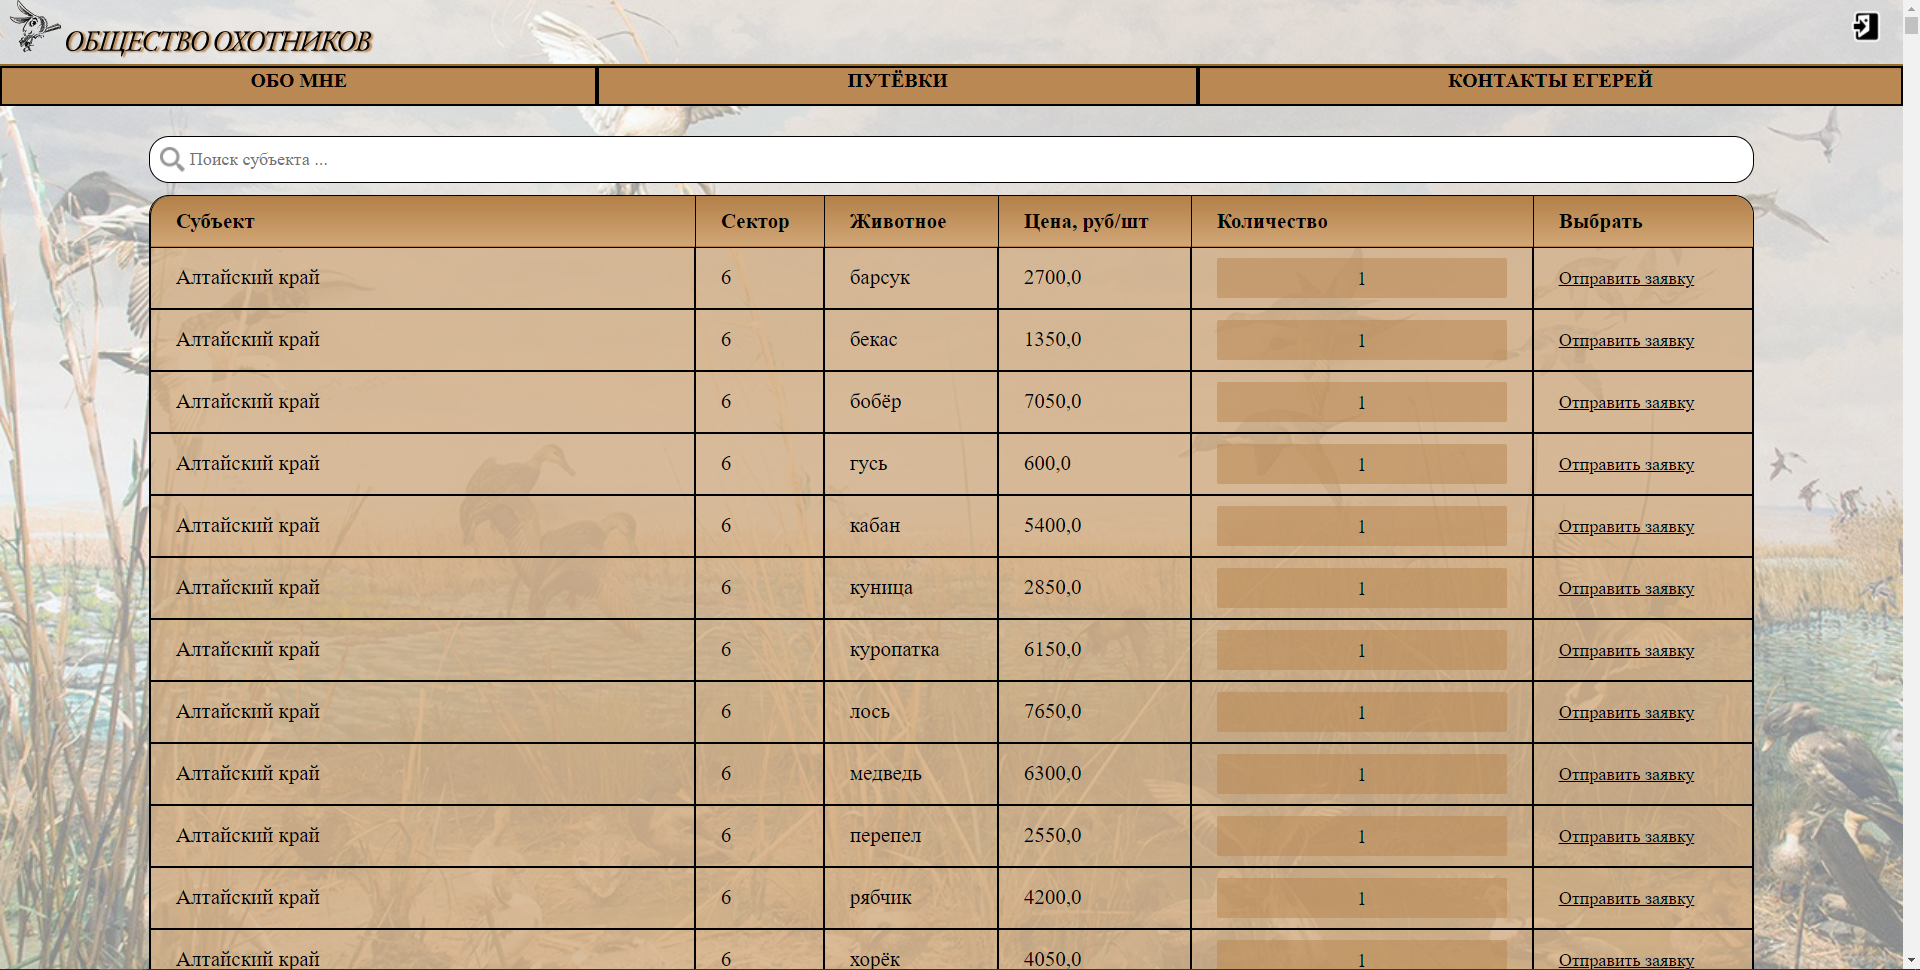
\includegraphics[scale=0.34]{schemes/screens/menu.png}}
			\caption{Прайс-лист доступных путёвок}
			\label{fig11:image}
		\end{center}
	\end{figure}

	Если охотник введёт некорректные данные (например, как на рисунке \ref{fig12:image}) и попробует оформить путёвку, нажав на <<Отправить заявку>>, то он увидит сообщение о невалидности данных (рисунок \ref{fig13:image}).
	
	\begin{figure}[h]
		\centering
		\begin{center}
			{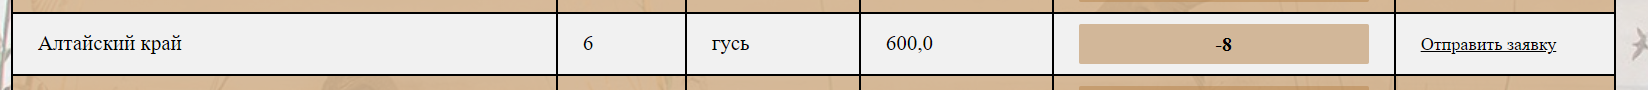
\includegraphics[scale=0.34]{schemes/screens/wrong_num.png}}
			\caption{Некорректный ввод данный в поле <<Количество>>}
			\label{fig12:image}
		\end{center}
	\end{figure}

	\begin{figure}[h]
		\centering
		\begin{center}
			{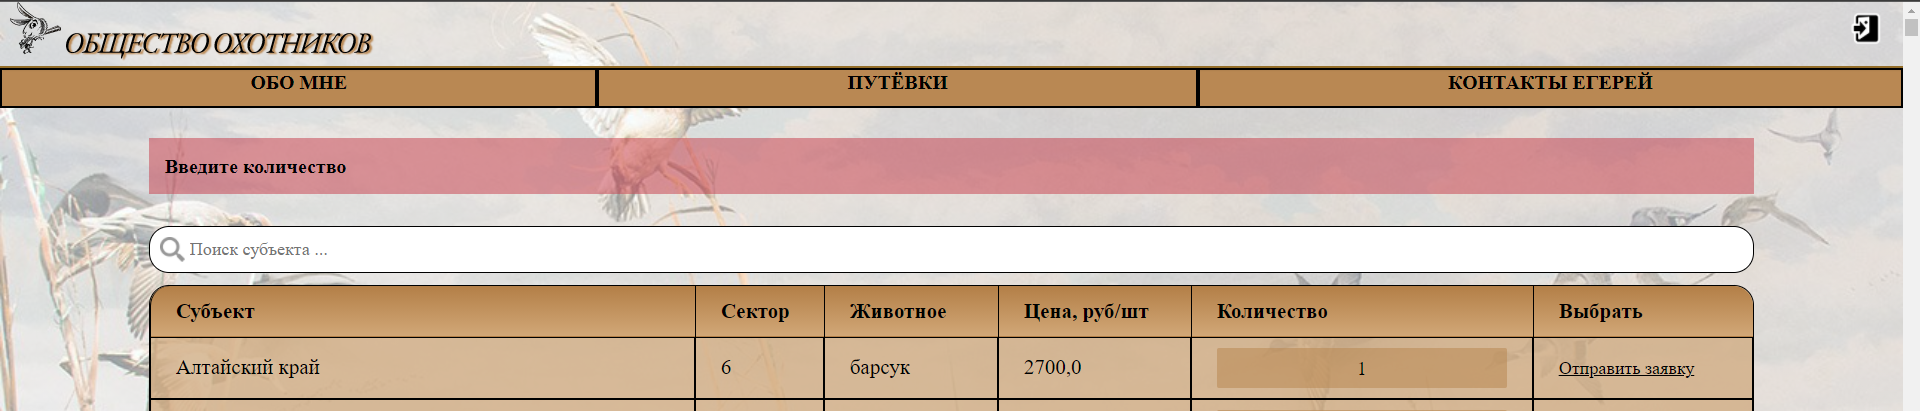
\includegraphics[scale=0.34]{schemes/screens/msg_error.png}}
			\caption{Сообщение о некорректном вводе данных}
			\label{fig13:image}
		\end{center}
	\end{figure}
	\newpage
	
	Также пользователь может воспользоваться поиском по названию субъекта (рисунок \ref{fig14:image}).
	
	\begin{figure}[h]
		\centering
		\begin{center}
			{
\includegraphics[scale=0.3245]{schemes/screens/find.png}}
			\caption{Демонстрация работы поиска}
			\label{fig14:image}
		\end{center}
	\end{figure}
	\newpage

	Если же охотник ввёл корректное число животных (рисунок \ref{fig15:image}) и нажал на <<Отправить заявку>>, то в этом случае на странице появляется соответствующее сообщение, как на рисунке \ref{fig16:image}.
	
	\begin{figure}[h]
		\centering
		\begin{center}
			{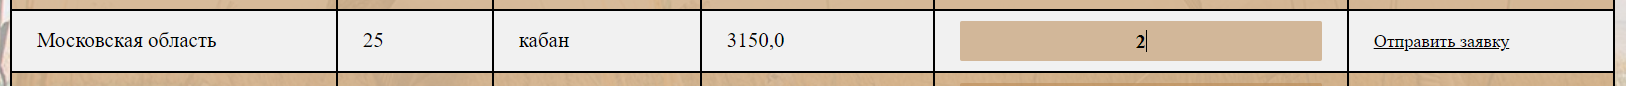
\includegraphics[scale=0.34]{schemes/screens/right_data.png}}
			\caption{Корректно оформленная заявка}
			\label{fig15:image}
		\end{center}
	\end{figure}

	\begin{figure}[h]
		\centering
		\begin{center}
			{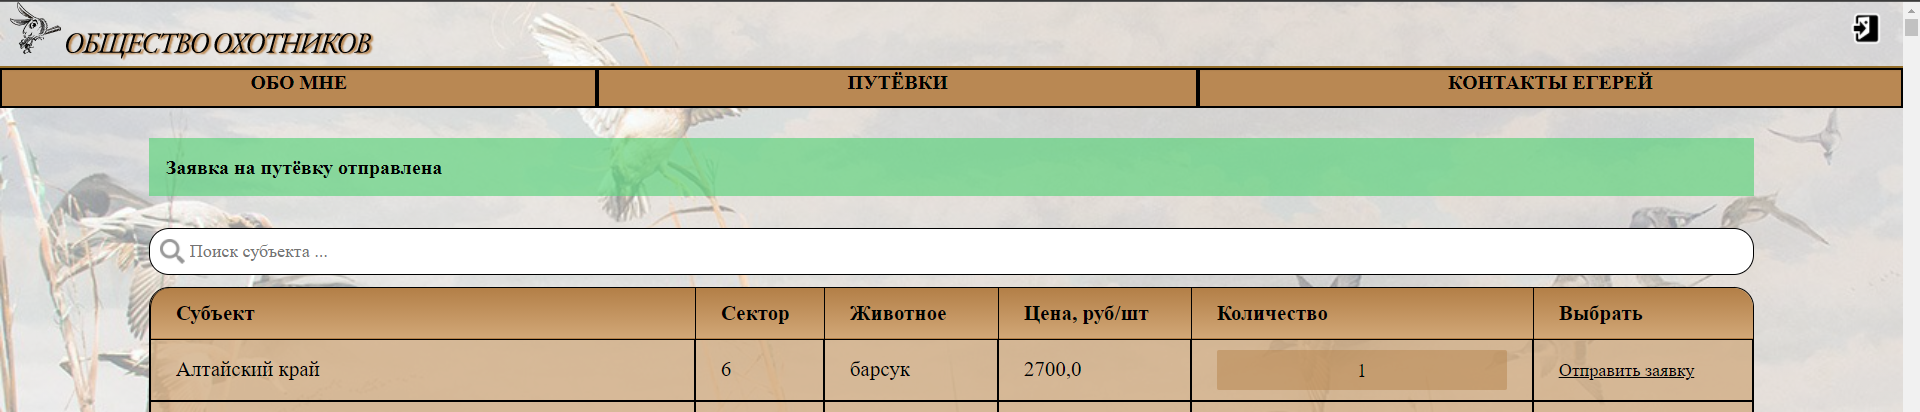
\includegraphics[scale=0.34]{schemes/screens/msg_right.png}}
			\caption{Сообщение об успешном оформлении заявки}
			\label{fig16:image}
		\end{center}
	\end{figure}

	Просмотреть все свои заявки, а также уже одобренные путёвки охотник может, кликнув на поле <<Просмотреть свои>> (рисунок \ref{fig17:image}).
	
	\begin{figure}[h]
		\centering
		\begin{center}
			{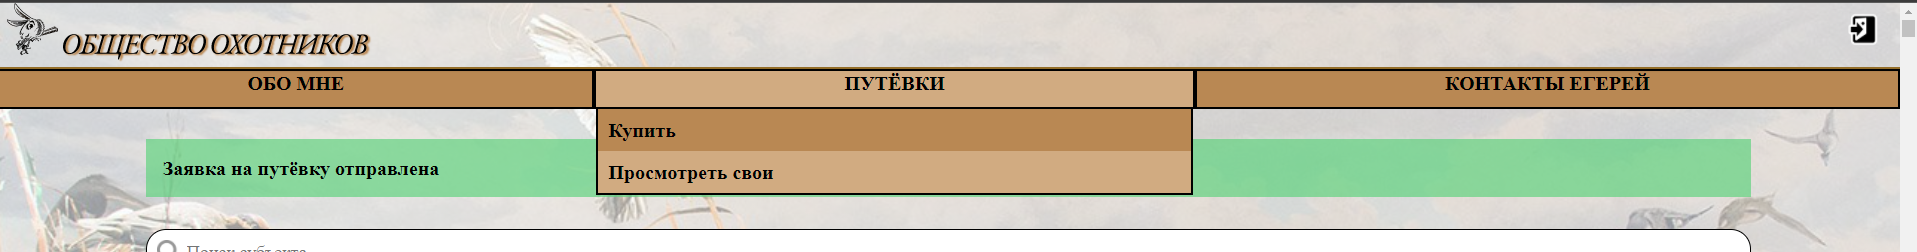
\includegraphics[scale=0.34]{schemes/screens/to_have.png}}
			\caption{Переход на страницу всех заявок и одобренных путёвок}
			\label{fig17:image}
		\end{center}
	\end{figure}

	В результате охотник попадает на страницу, изображённую на рисунке \ref{fig18:image}. На ней сначала указаны все одобренные текущему охотнику путёвки (то есть, по ним он уже может охотиться), и ниже все заявки. Также по каждой из этих двух таблиц можно осуществить поиск по субъекту. На рисунке \ref{fig15:image} указано, какая именно позиция из прайс-листа была выбрана, и уже на этой странице можно увидеть эту заявку (выделена белым цветом).
	
	\begin{figure}[h]
		\centering
		\begin{center}
			{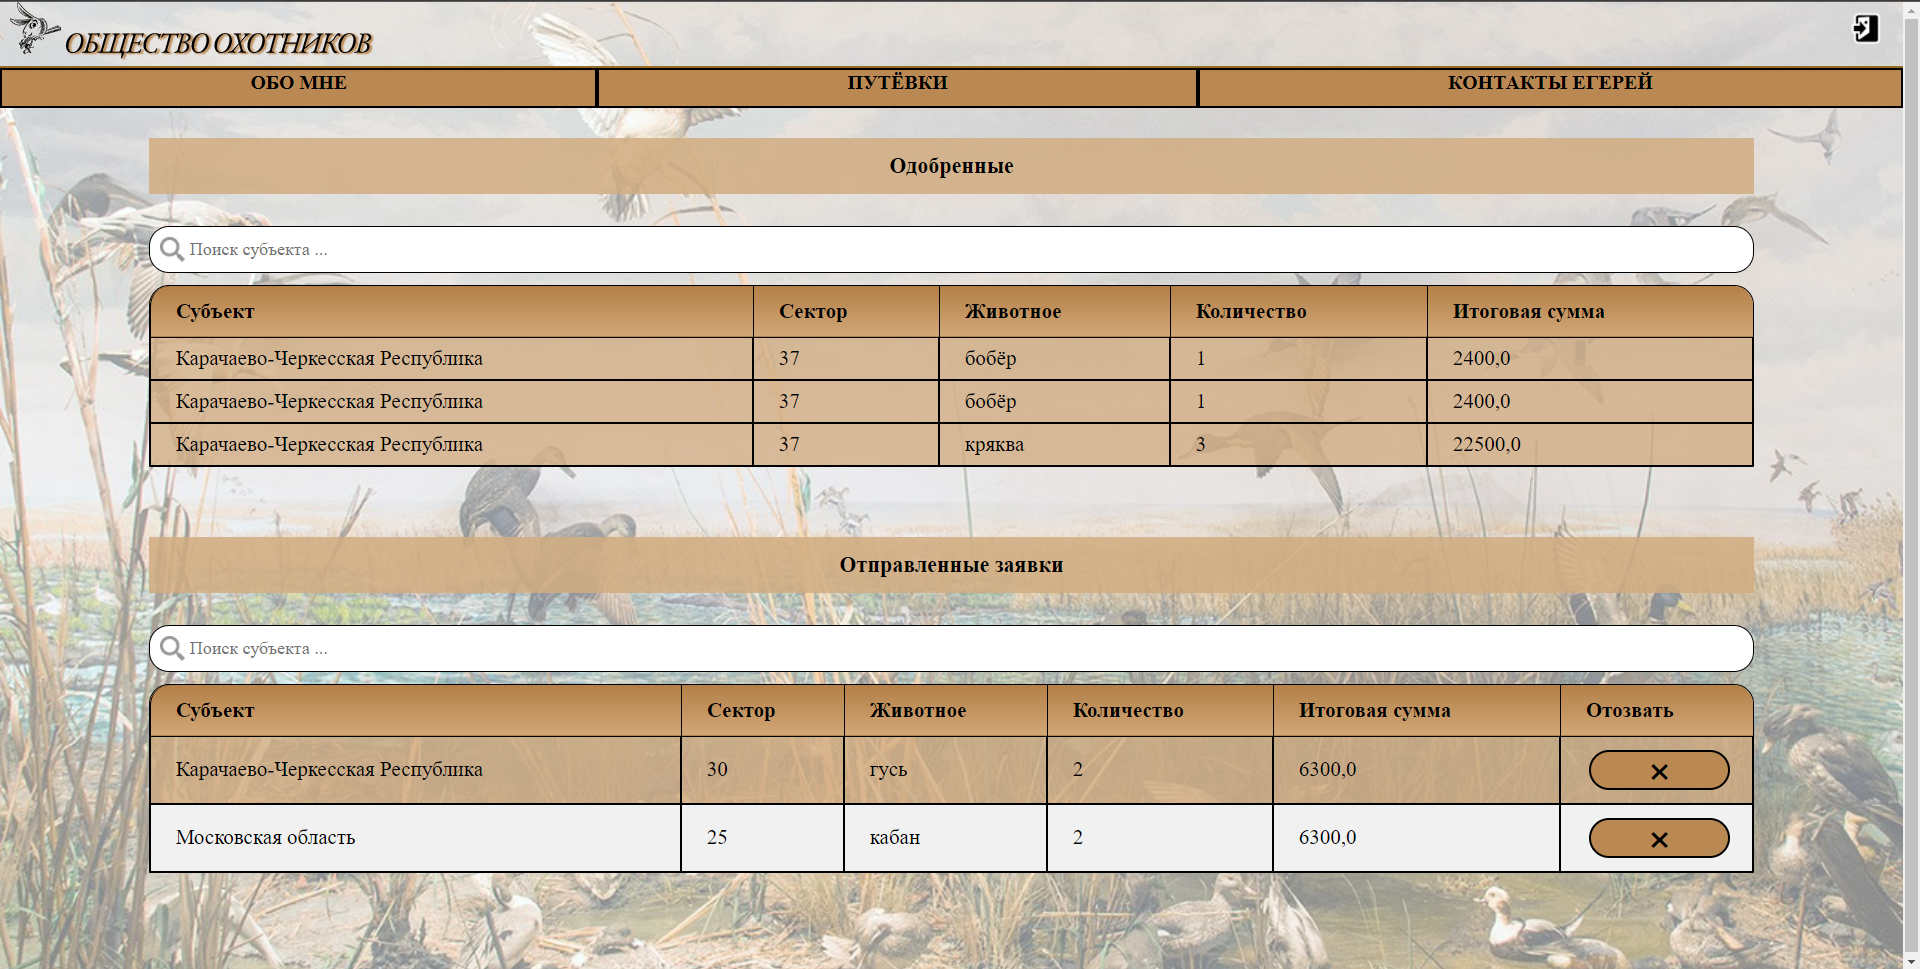
\includegraphics[scale=0.34]{schemes/screens/all_vouchers.png}}
			\caption{Всех заявки и одобренные путёвок текущего охотника}
			\label{fig18:image}
		\end{center}
	\end{figure}

	Если по какой-то причине пользователь передумал оформлять путёвку, то он может отозвать оформленную ранее заявку, нажав на кнопку в столбце <<Отозвать>>. 
	
	Для наглядности была отозвана путёвка на гуся. После этого страница выглядит так, как показано на рисунке \ref{fig19:image}. 
	
	Показателем того, что операция прошла успешно, является соответствующее сообщение и отсутствие выбранной позиции на странице. 
	
	Удалить или отозвать уже одобренные путёвки охотник не может, так как считается, что покупка уже совершена, а закрыть её по определённым причинам может только егерь, закреплённый за сектором, куда была выдана путёвка, или администратор.
	
	\begin{figure}[pt!]
		\centering
		\begin{center}
			{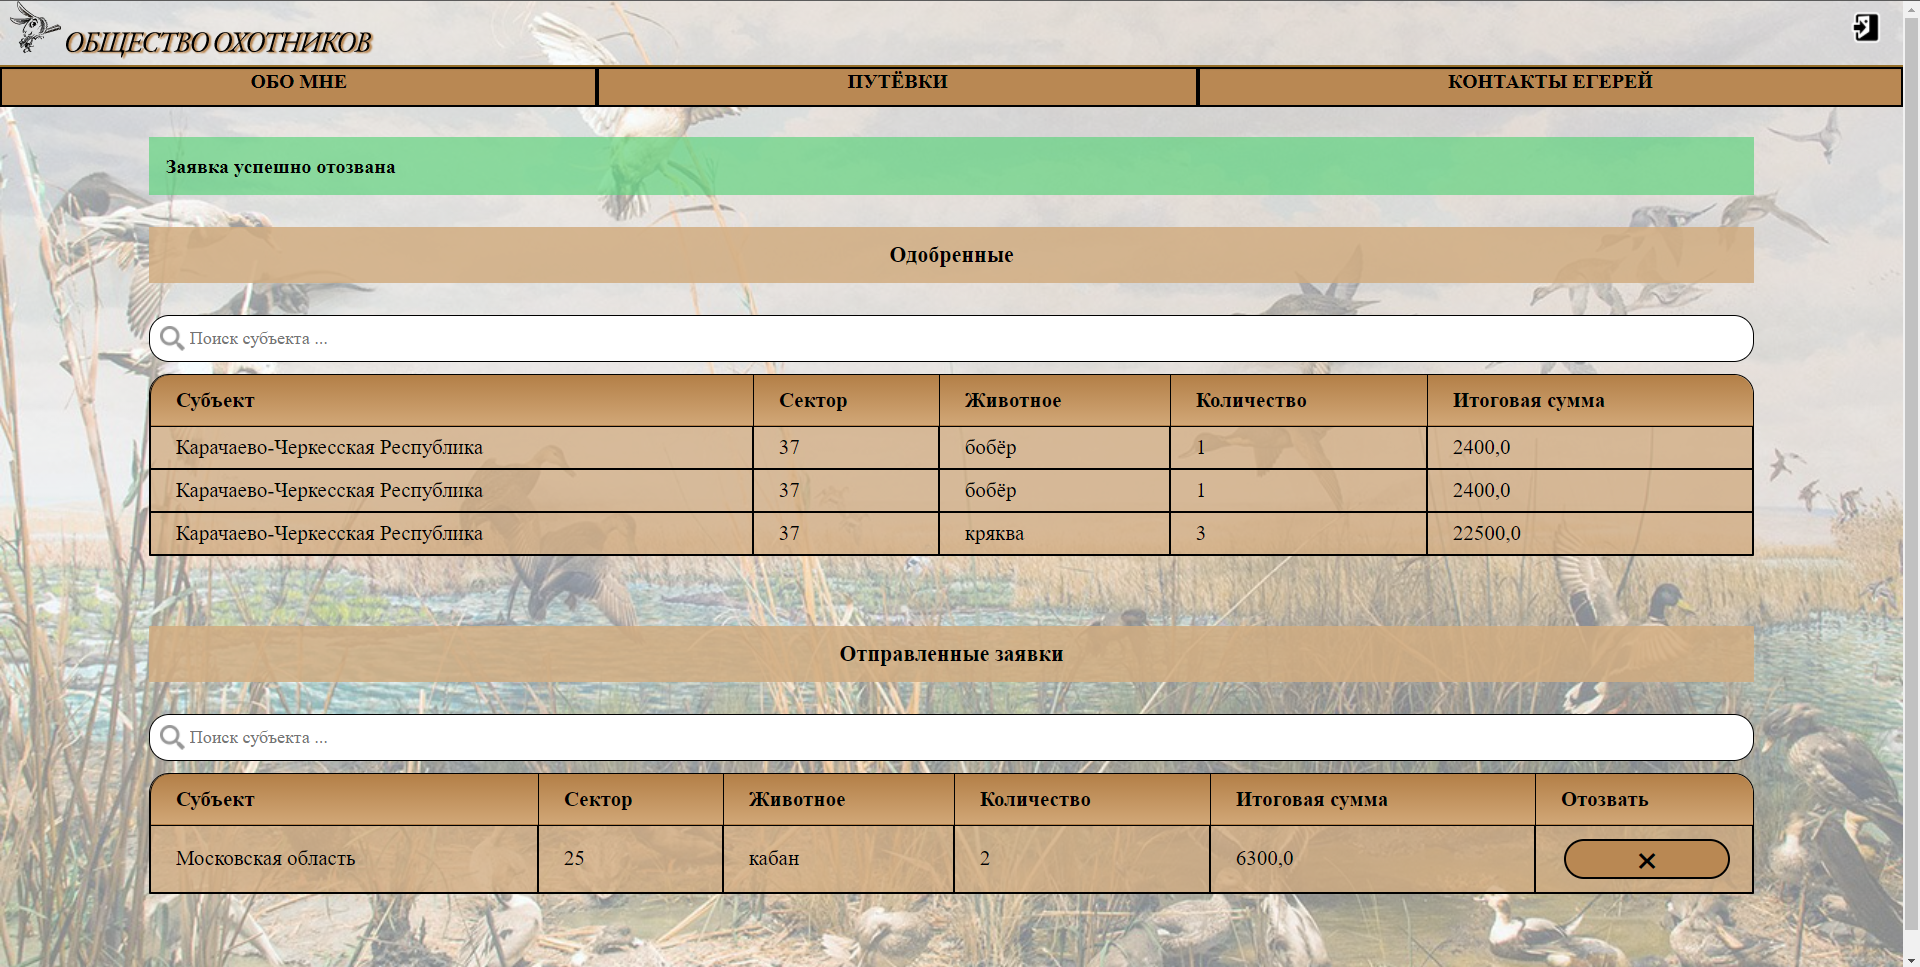
\includegraphics[scale=0.34]{schemes/screens/after_del_huntsman.png}}
			\caption{Страница после того, как была отозвана заявка}
			\label{fig19:image}
		\end{center}
	\end{figure}
	\newpage

	Также оперировать заявками на охоту и путёвками может и егерь. Для того, чтобы просмотреть заявки ему также нужно перейти по тому же пункту меню (рисунок \ref{fig20:image}). Стоит отметить, что видеть и проводить какие-либо операции егерь может только над теми заявками и путёвками, которые были оформлены в его хозяйство и сектор, к остальным данным он доступа не имеет.
	
	\begin{figure}[h]
		\centering
		\begin{center}
			{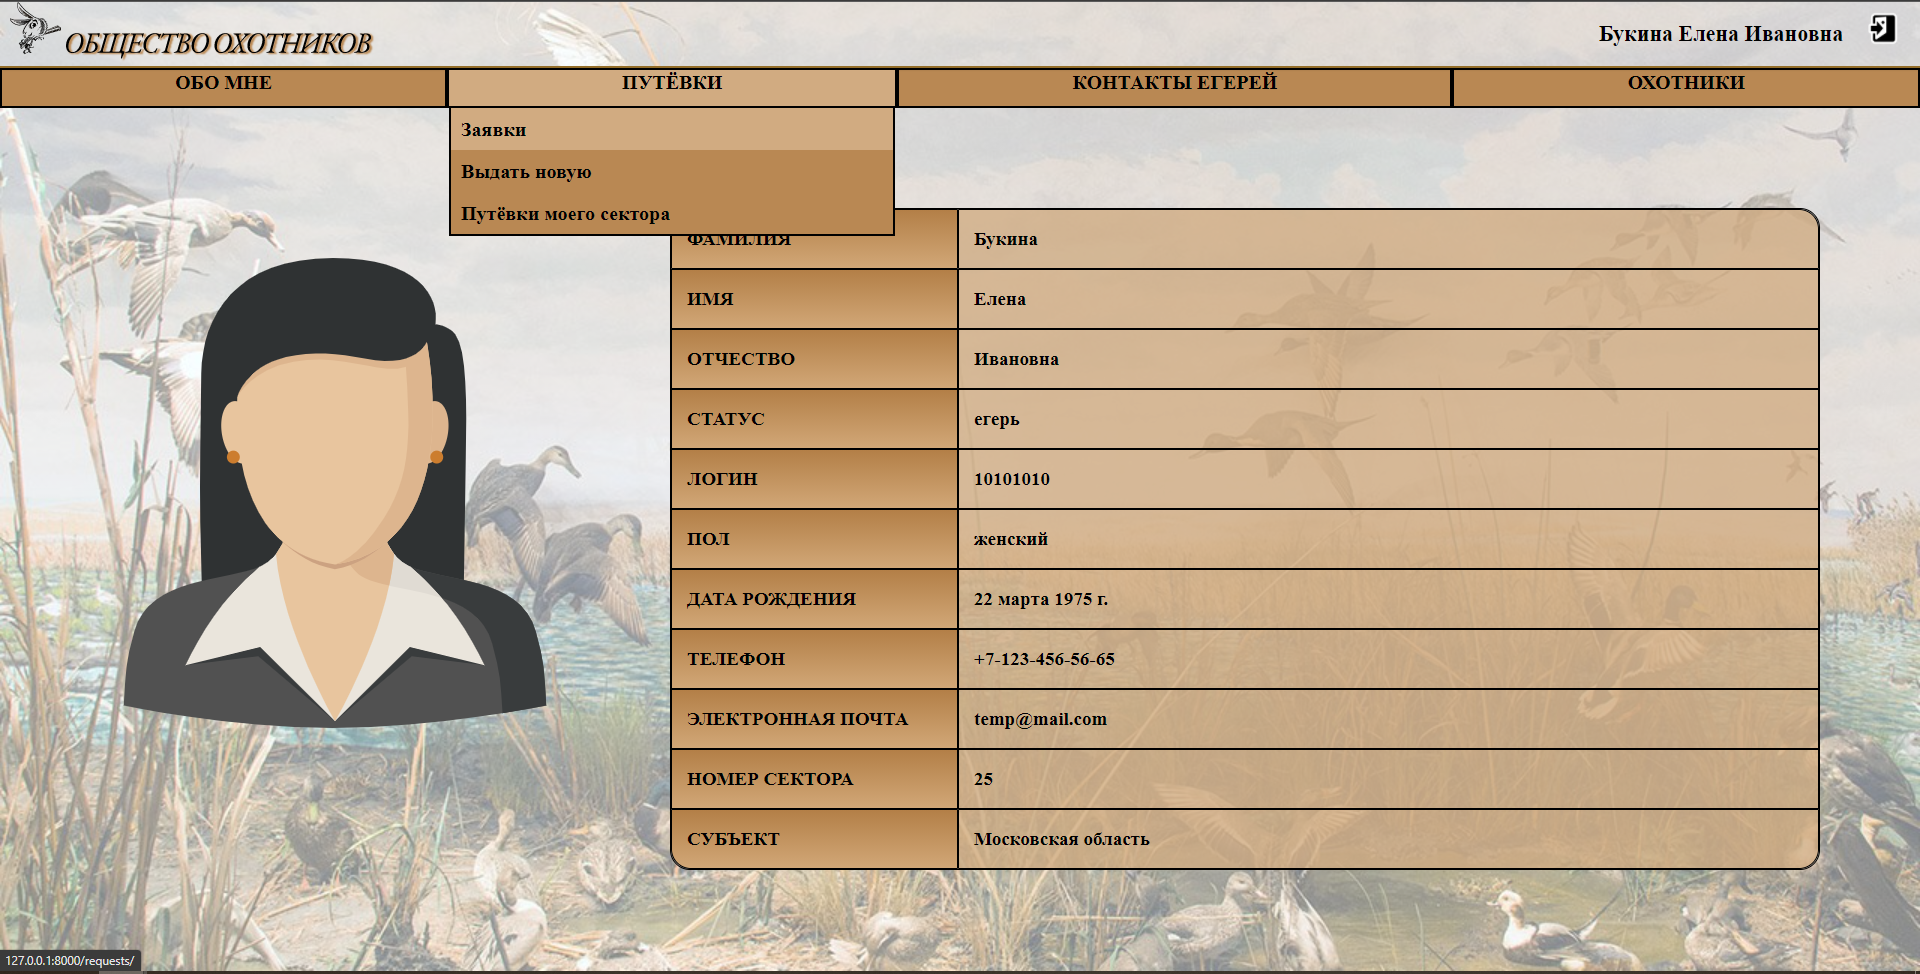
\includegraphics[scale=0.34]{schemes/screens/huntsman_start.png}}
			\caption{Переход на страницу заявок со стороны егеря}
			\label{fig20:image}
		\end{center}
	\end{figure}
	\newpage

	Страница заявок изображена на рисунке \ref{fig21:image}. Белым цветом выделена путёвка, которая оформлялось ранее. Егерь может как одобрить путёвку, нажав на <<галочку>>, так и отклонить, выбрав <<крестик>>. Также егерю предоставляется поиск по ФИО.

	\begin{figure}[h]
		\centering
		\begin{center}
			{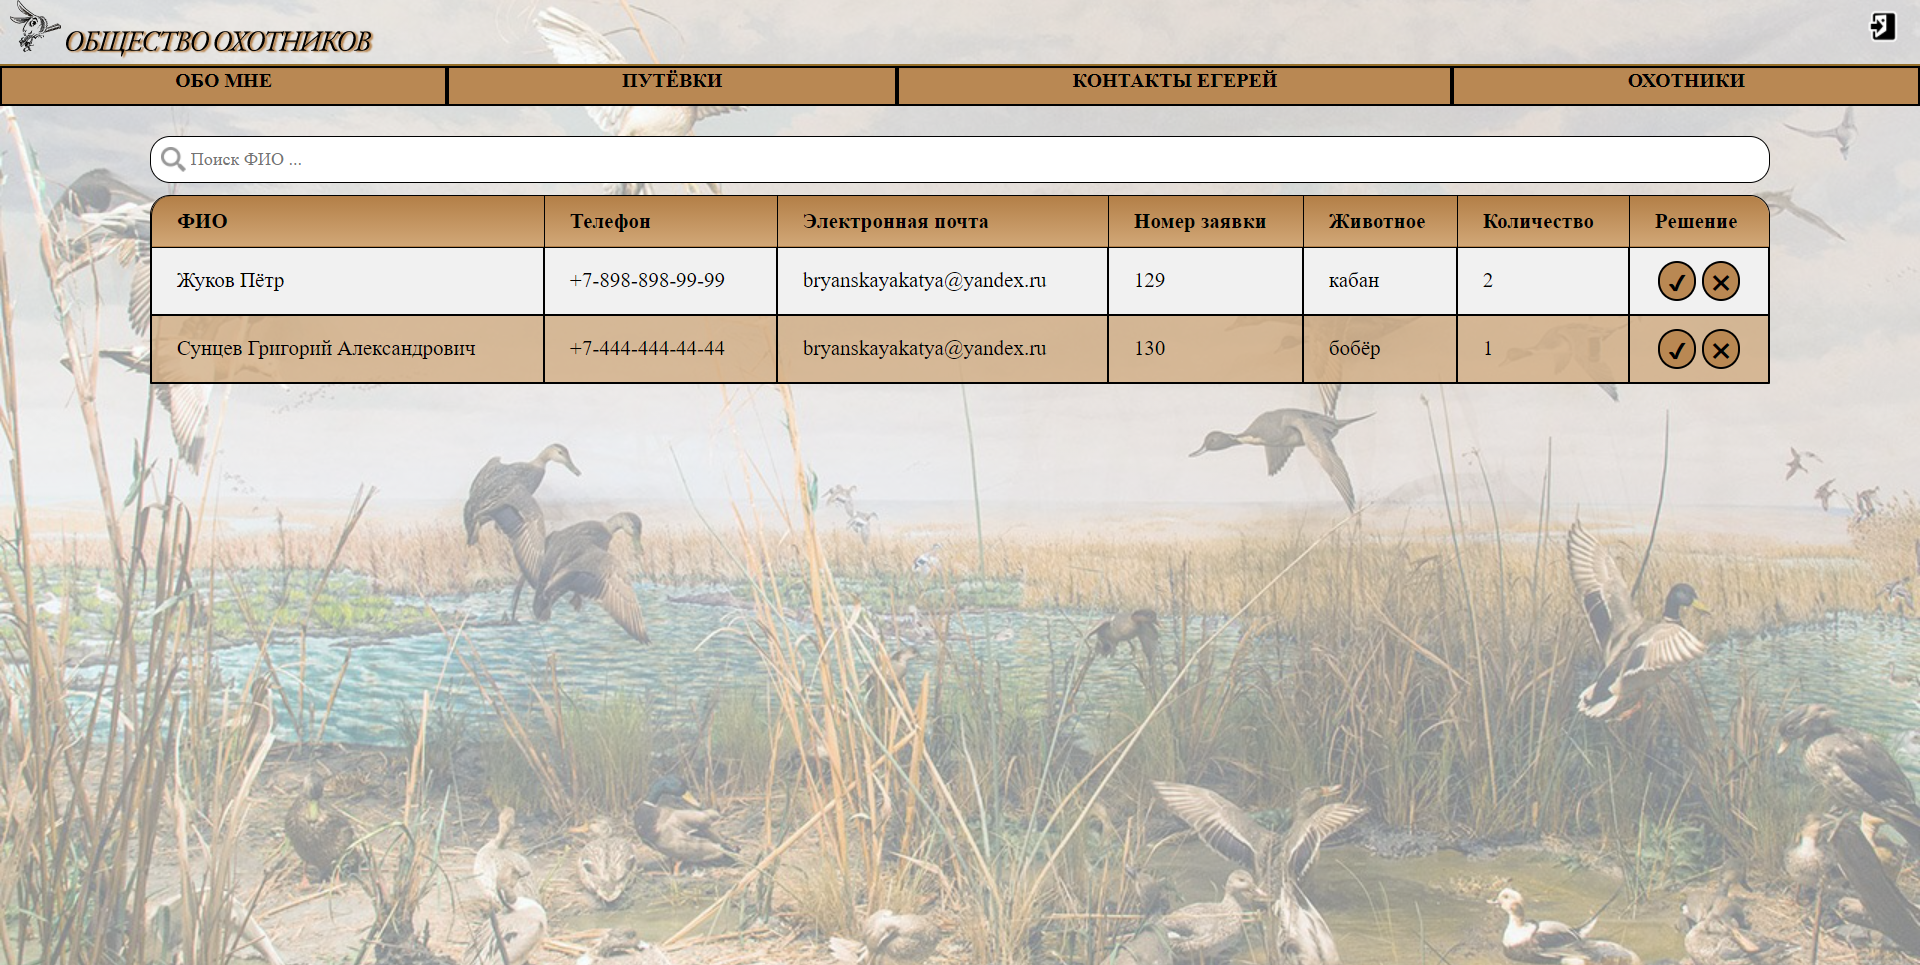
\includegraphics[scale=0.321]{schemes/screens/requests_huntsman.png}}
			\caption{Страница заявок, доступных егерю}
			\label{fig21:image}
		\end{center}
	\end{figure}

	Перейдя по пункту <<Путёвки моего сектора>> из меню (рисунок \ref{fig20:image}) на страницу, изображённую на рисунке \ref{fig23:image}, пользователь получает соответствующий список.
	
	\begin{figure}[h]
		\centering
		\begin{center}
			{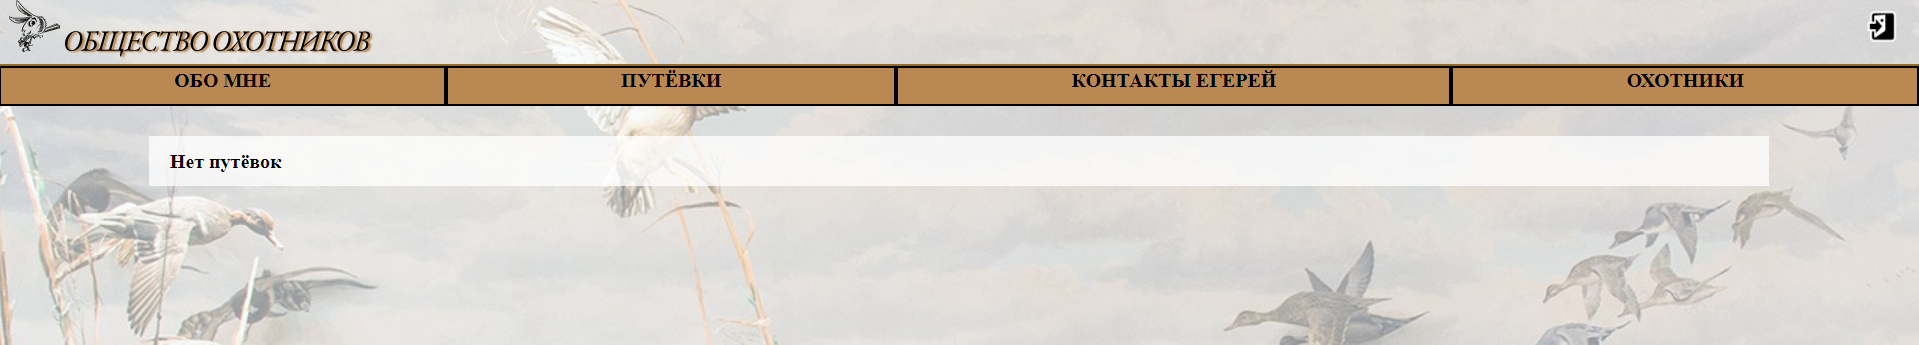
\includegraphics[scale=0.34]{schemes/screens/vouchers_huntsman2.png}}
			\caption{Страница одобренных путёвок, доступных егерю}
			\label{fig23:image}
		\end{center}
	\end{figure}
	\newpage

	На данный момент выданных путёвок нет. Если егерь примет решение одобрить путёвку на кабана (рисунок \ref{fig21:image}) и нажмёт <<галочку>>, то страницы заявок (рисунок \ref{fig24:image}) и путёвок (рисунок \ref{fig25:image}) примут соответствующий вид.
	
	\begin{figure}[h!]
		\centering
		\begin{center}
			{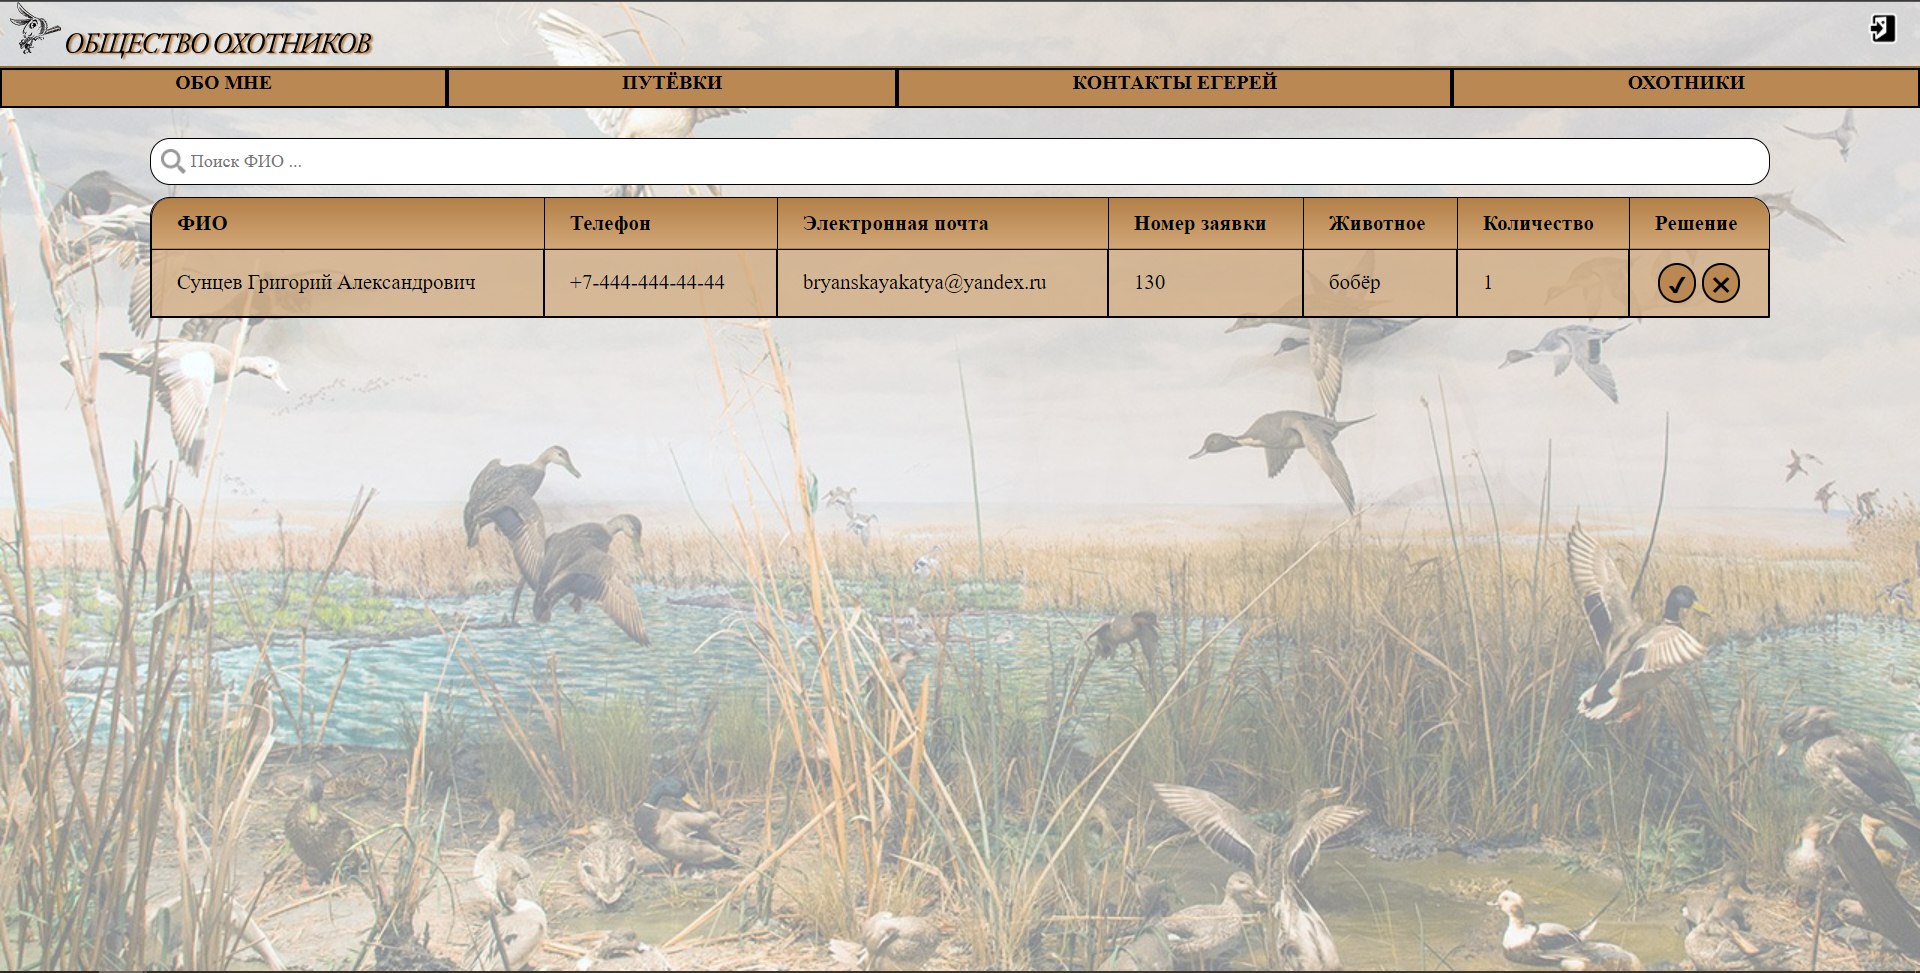
\includegraphics[scale=0.34]{schemes/screens/requests_huntsman_add.png}}
			\caption{Страница заявок, доступных егерю, после одобрения}
			\label{fig24:image}
		\end{center}
	\end{figure} 

	\begin{figure}[pt!]
		\centering
		\begin{center}
			{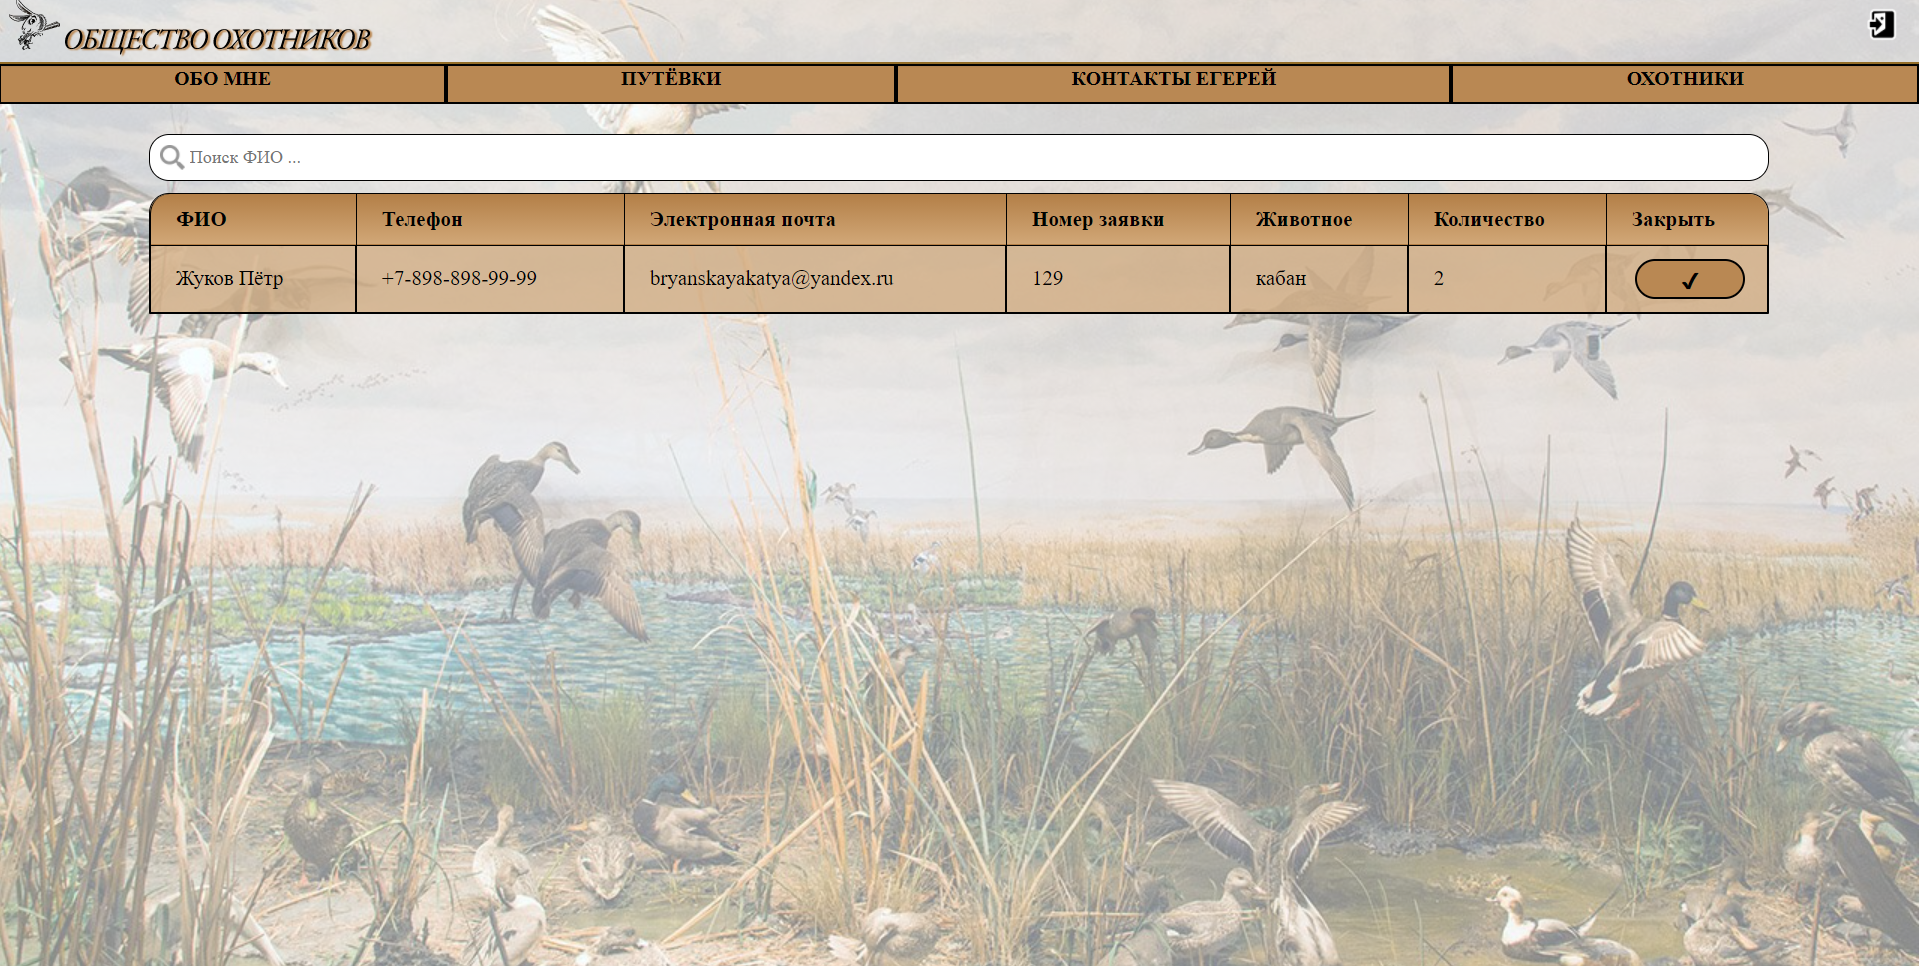
\includegraphics[scale=0.34]{schemes/screens/vouchers_huntsman_add.png}}
			\caption{Страница одобренных путёвок, доступных егерю, после одобрения}
			\label{fig25:image}
		\end{center}
	\end{figure} 
	\newpage

	Оформленная ранее путёвка теперь числится не в ожидающий заявках, а в одобренных путёвках.
	
	Егерь также может закрыть путёвку (например, при её истечении), для этого он должен нажать на соответствующую кнопку в столбце <<Закрыть>> на странице путёвок (рисунок \ref{fig25:image}), и данная позиция перестанет существовать.
	
	Егерь также может принять решение об отказе на оформление путёвки, для этого он нажимает <<крестик>> (рисунок \ref{fig24:image}). В такой ситуации путёвка пропадёт не только у егеря, но и у охотника, на чьё имя она была оформлена.\\

	Помимо этого егерь может выдать кому-то путёвку, но только в то хозяйствой и сектор, к которому прикреплён сам. В таком случае, оформленная путёвка сразу получает статус одобренной и попадает в соответствующий раздел. Чтобы перейти на страницу оформления путёвки, нужно выбрать пункт <<Выдать новую>> из меню (рисунок \ref{fig20:image}). Егерь в таком случае попадает на страницу, приведённую на рисунке \ref{fig28:image}.

	\begin{figure}[h]
		\centering
		\begin{center}
			{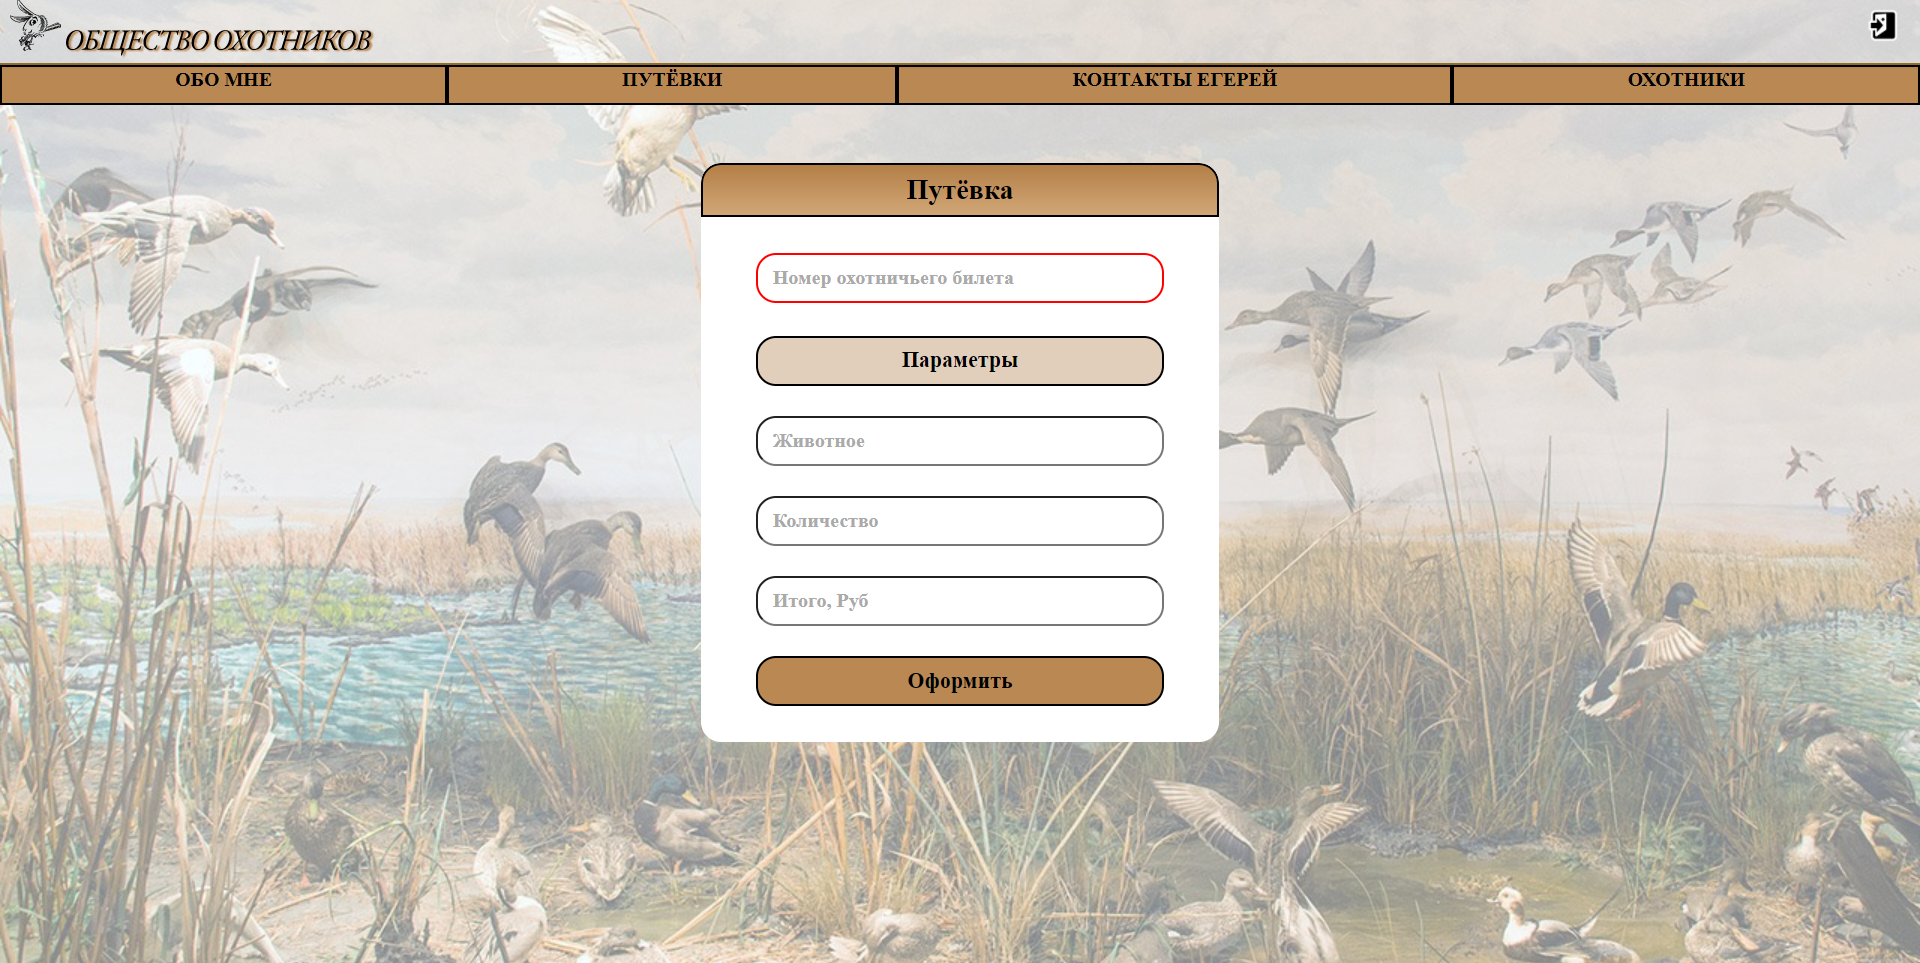
\includegraphics[scale=0.34]{schemes/screens/create_huntsman.png}}
			\caption{Оформление путёвки егерем}
			\label{fig28:image}
		\end{center}
	\end{figure}
	\newpage

	Помимо поля, предназначенного для ввода номера охотничьего билета, необходимо также выбрать параметры. Делается это по нажатию на одноимённую кнопку. В результате егерю предоставляется весь прайс-лист, действующий в его секторе (рисунок \ref{fig29:image}).
	
	\begin{figure}[h!]
		\centering
		\begin{center}
			{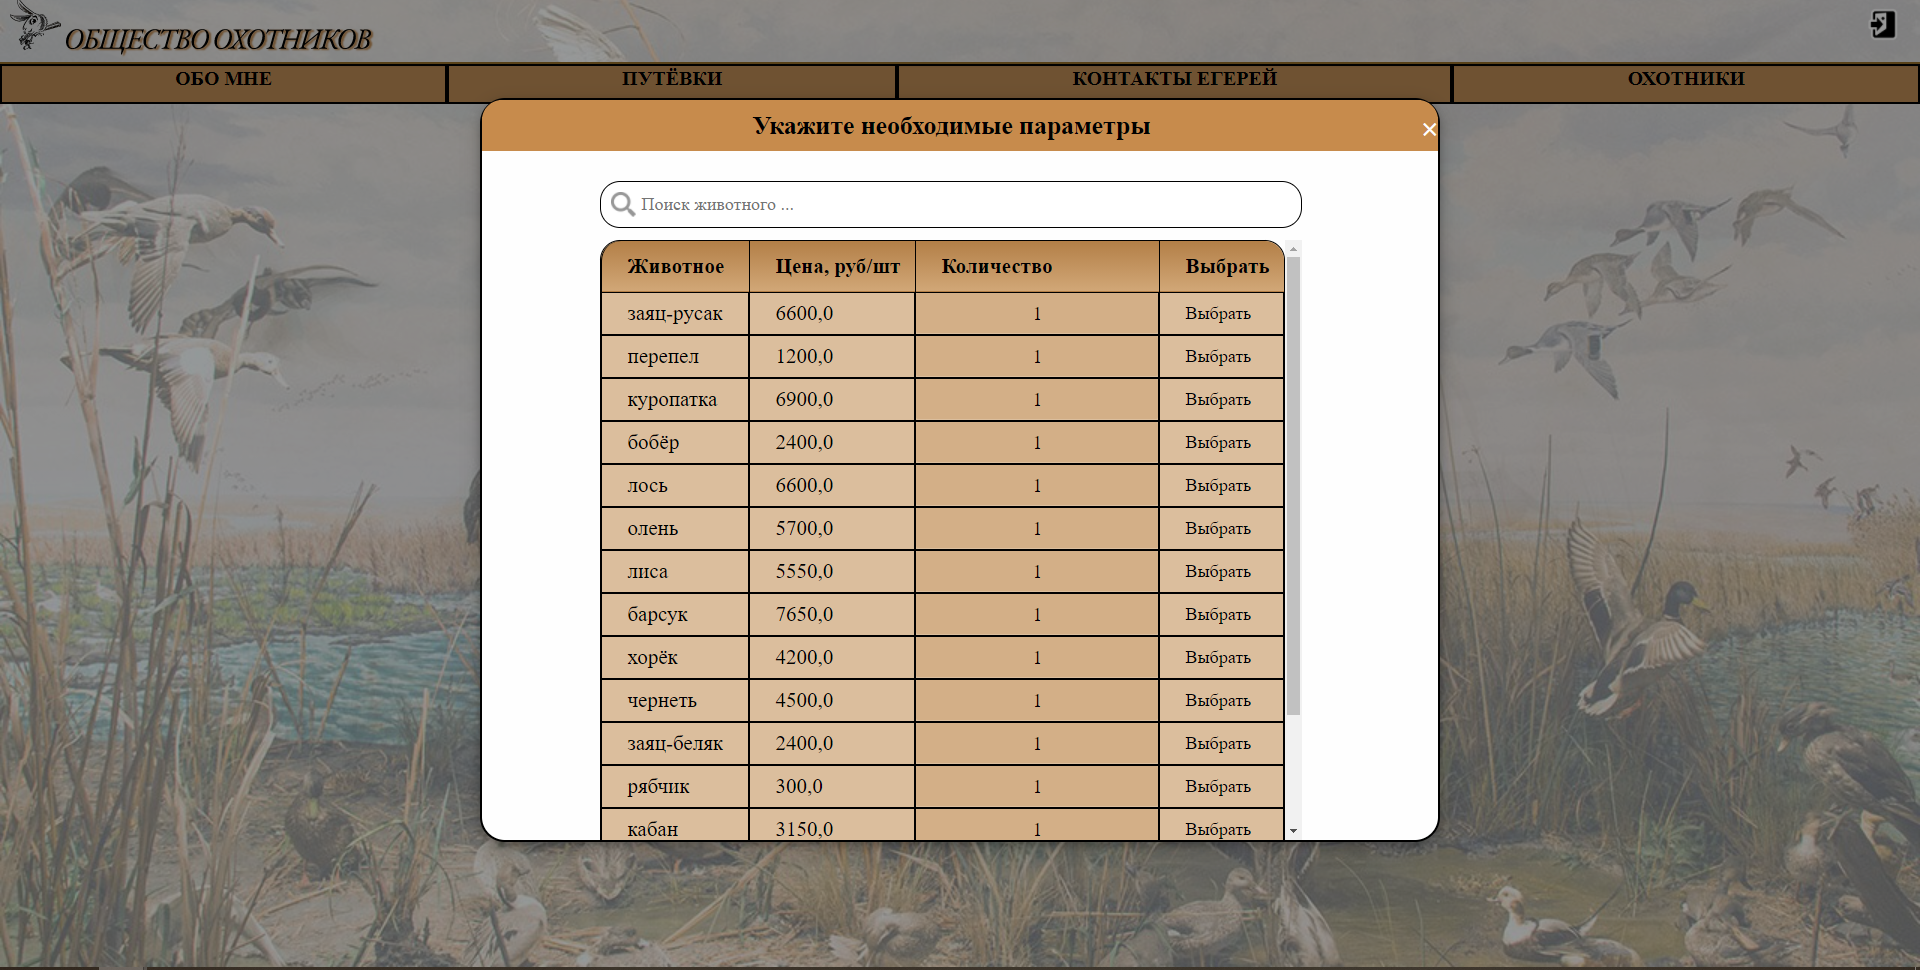
\includegraphics[scale=0.34]{schemes/screens/price_list_huntsman.png}}
			\caption{Выбор параметров путёвки}
			\label{fig29:image}
		\end{center}
	\end{figure}

	Здесь также предусмотрен поиск по названию животного, а также проверка на валидность введенного количества, аналогичная той, что была ранее.
	
	Заполнив поля (рисунок \ref{fig28:image}) и нажав кнопку <<Оформить>> может возникнуть одна из двух ситуаций. Первая - когда всё верно, и в базе действительно существует охотник с указанным билетом, в таком случае, егерь просто попадает на страницу разрешённых путёвок и наблюдает там только что оформленную путёвку. И вторая - охотника с таким номером нет, в таком случае, просто выводится ошибка на экран.
	
	Что касается администратора, то он может выполнять те же операции над заявками и путёвками, что и егерь, с той лишь разницей, что ему предоставляются данные со всех хозяйств и секторов. Так, страницы заявок (рисунок \ref{fig31:image}) и одобренных путёвок (рисунок \ref{fig32:image}) со стороны администратора отличаются только наличием столбцов о месте проведения, функционал такой же.
	
	\begin{figure}[h!]
		\centering
		\begin{center}
			{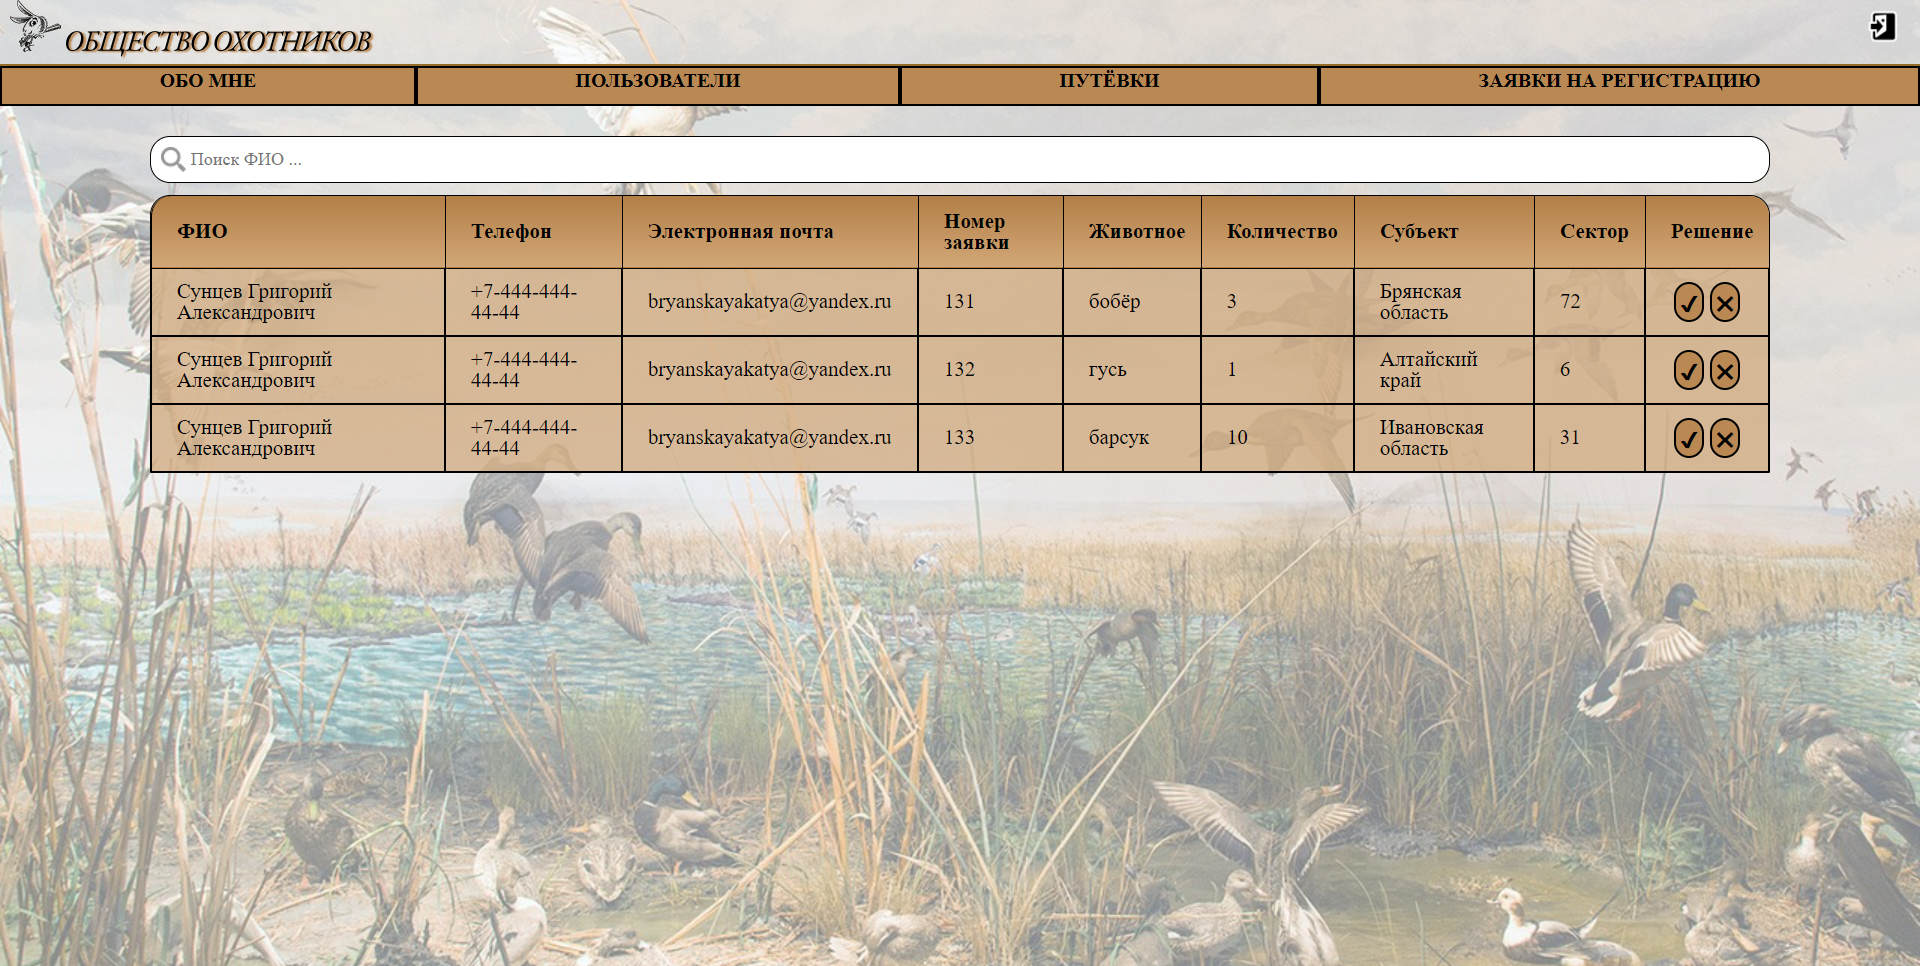
\includegraphics[scale=0.34]{schemes/screens/requests_admin.png}}
			\caption{Страница заявок со стороны администратора}
			\label{fig31:image}
		\end{center}
	\end{figure}

	\begin{figure}[h!]
		\centering
		\begin{center}
			{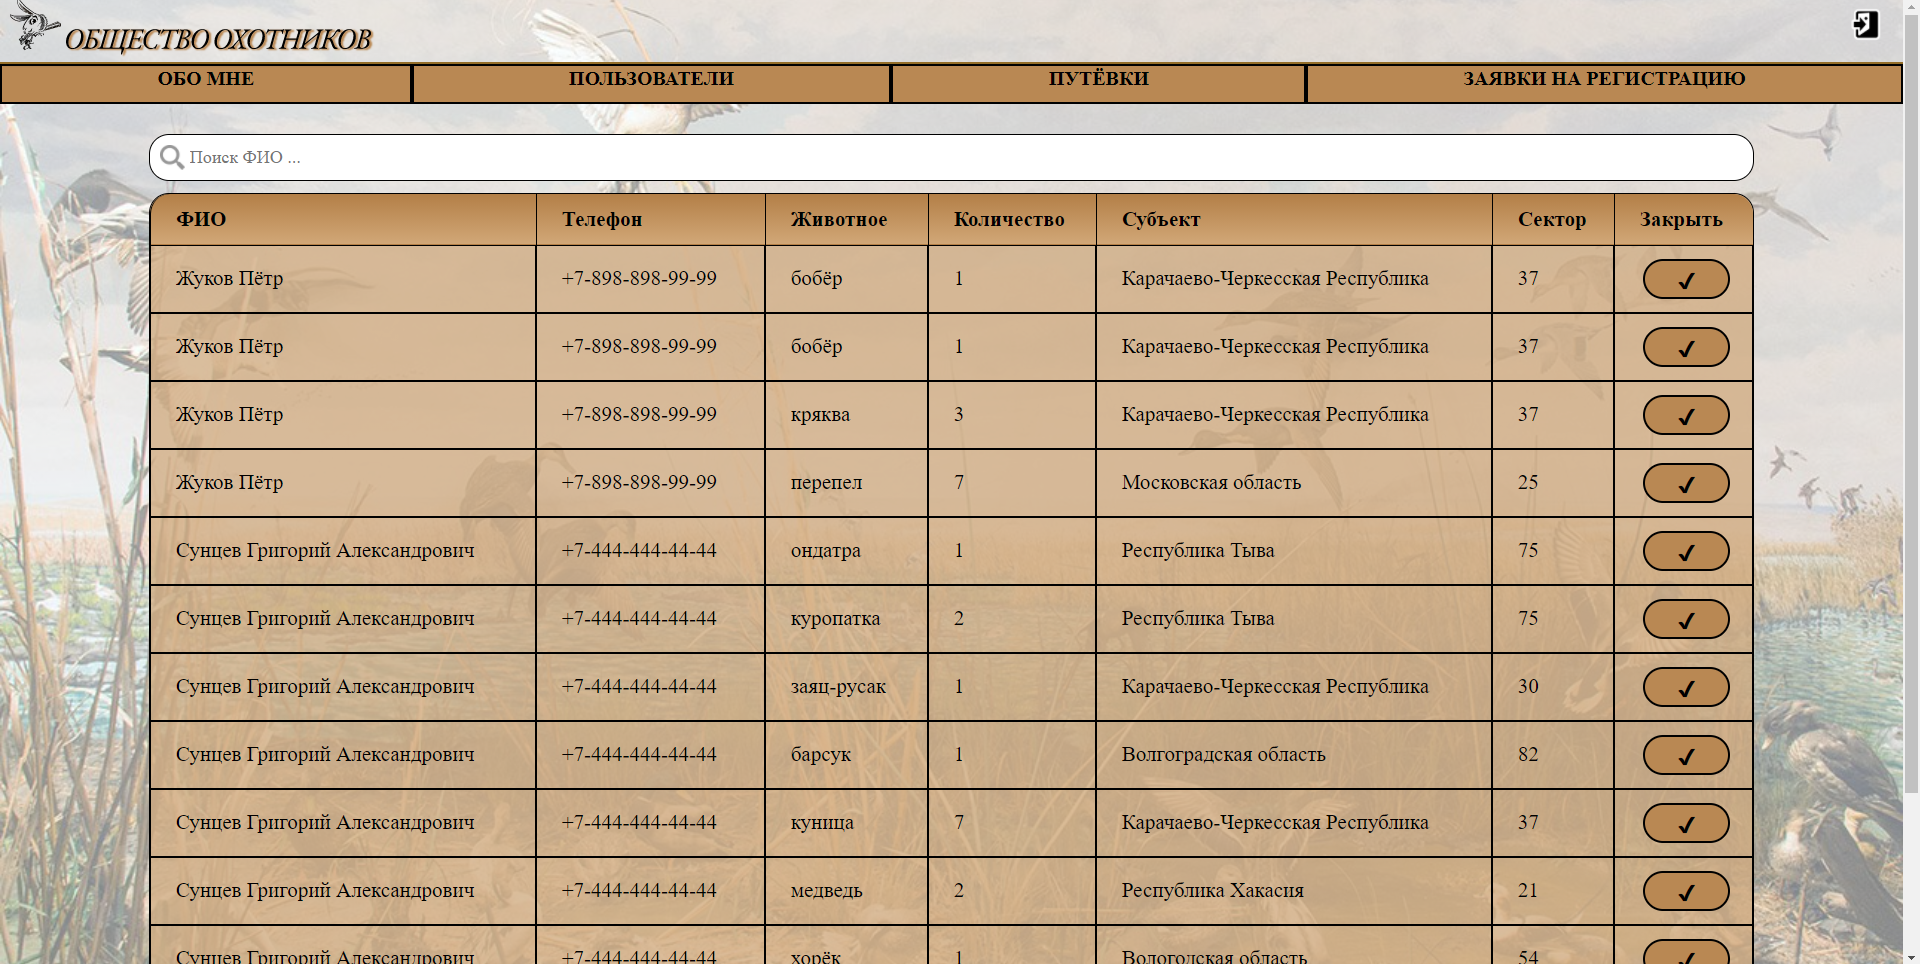
\includegraphics[scale=0.34]{schemes/screens/vouchers_admin.png}}
			\caption{Страница одобренных путёвок со стороны администратора}
			\label{fig32:image}
		\end{center}
	\end{figure}
	\newpage

	Возможность оформления путёвки через администратора тоже есть, он также должен заполнить форму, аналогичную изображенной на рисунке \ref{fig30:image}, только теперь  ещё надо заполнить поле о месте проведения (рисунок \ref{fig33:image}).
	
	\begin{figure}[h!]
		\centering
		\begin{center}
			{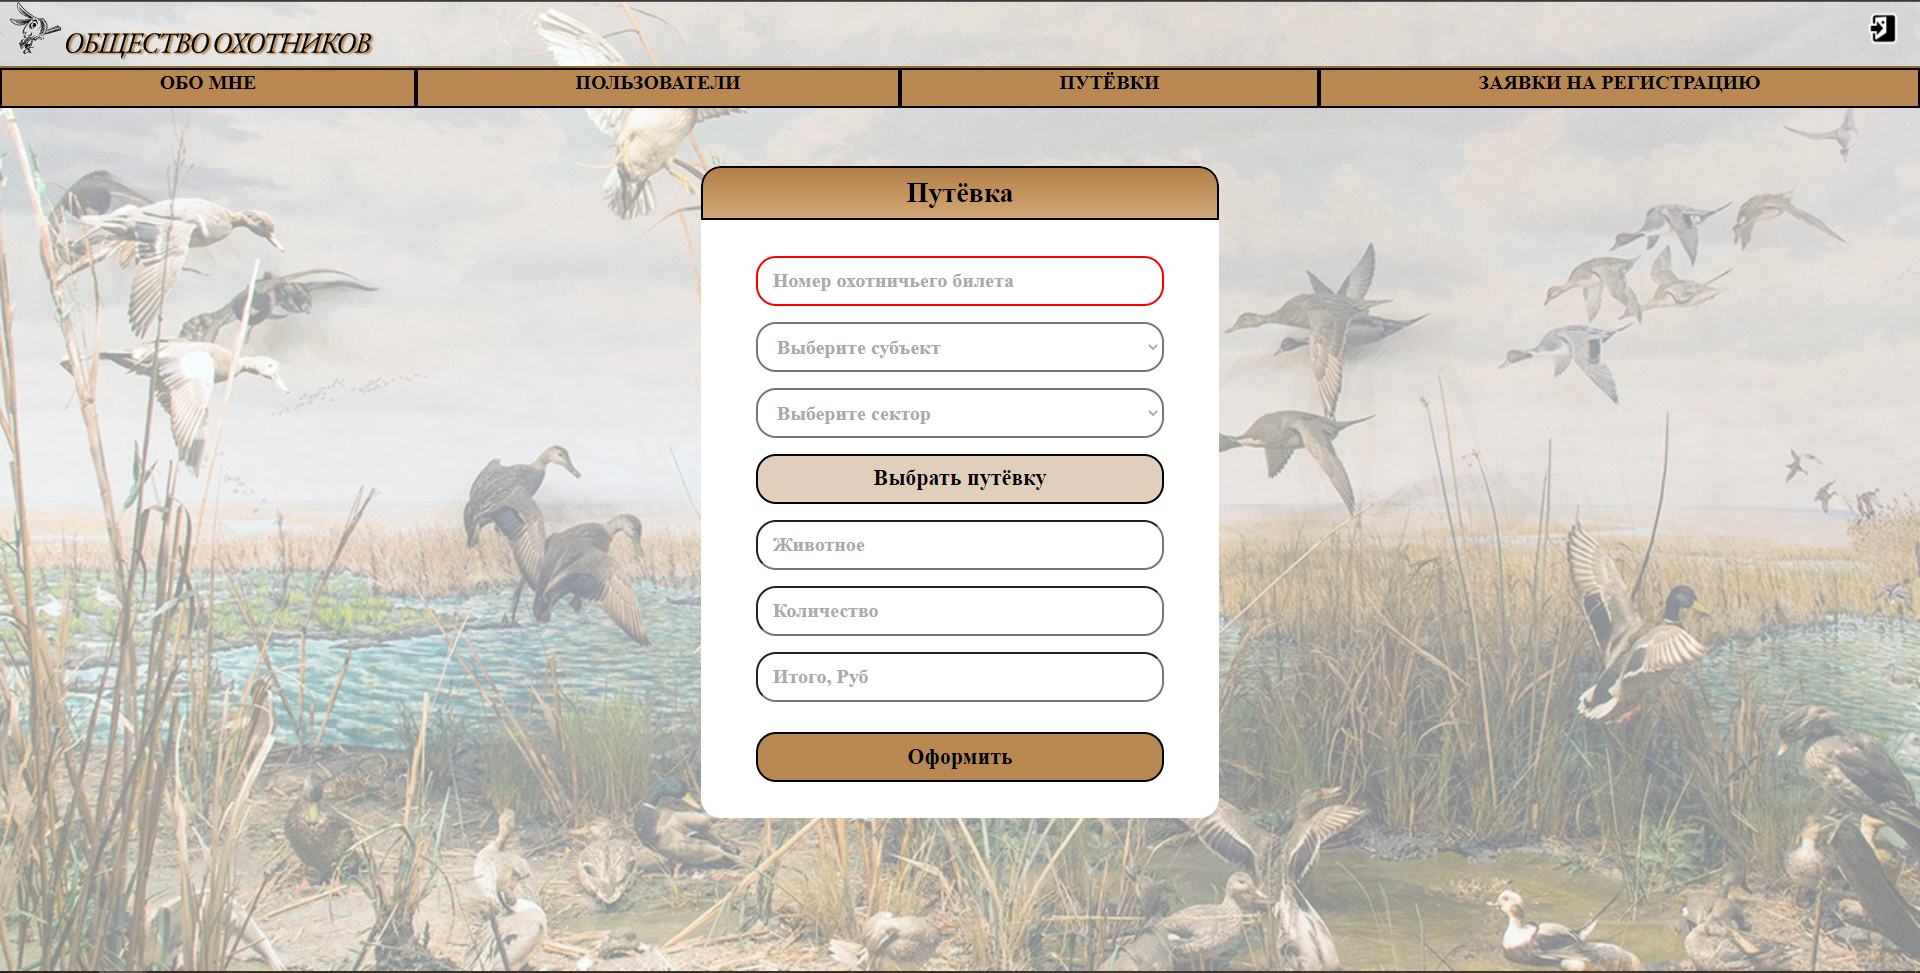
\includegraphics[scale=0.34]{schemes/screens/create_admin.png}}
			\caption{Оформление путёвки администратором}
			\label{fig33:image}
		\end{center}
	\end{figure}
	\newpage

	Поля <<Выберите субъект>> и <<Выберите сектор>> представляют из себя выпадающие списки (рисунок \ref{fig34:image}). Это сделано для того, чтобы минимизировать количество вводимых с клавиатуры данных, с целью сократить число возникающих в ходе заполнения ошибок.
	
	\begin{figure}[h!]
		\centering
		\begin{center}
			{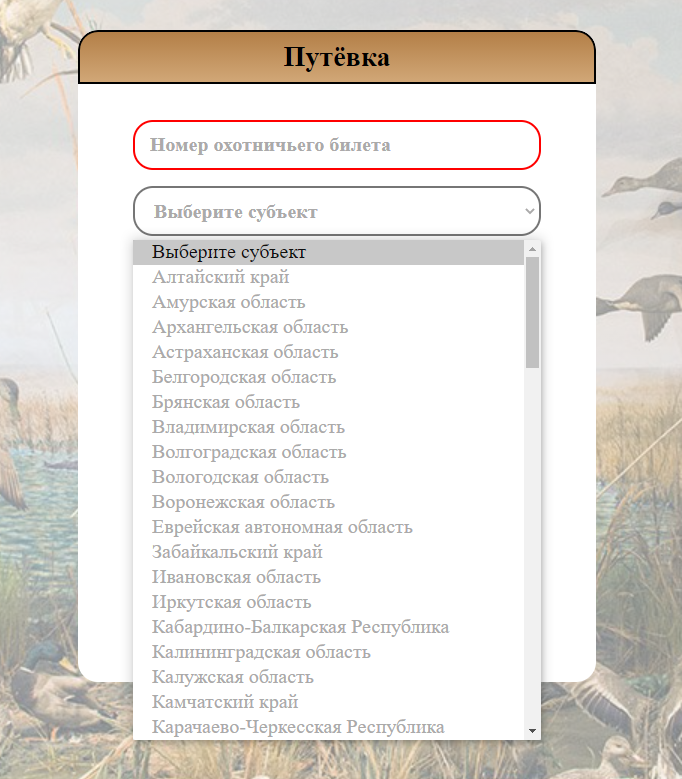
\includegraphics[scale=0.5]{schemes/screens/scroll_menu.png}}
			\caption{Выпадающий список}
			\label{fig34:image}
		\end{center}
	\end{figure}
	
	\subsection*{Вывод}
	Для реализации поставленной задачи были выбраны язык программирования Python и среды разработки Pycharm и Visual Studio Code.
	
	В качестве используемых СУБД и ORM были выбраны PostgreSQL и peewee, а для разработки Web-фреймворка - Django.
	
	В разделе также были представлены в виде UML-диаграмм компонент доступа к данным, компонент бизнес-логики, представления, а также общая диаграмма приложения.
	
	Был также освещён интерфейс приложения, задействованный при оформлении разными ролями путёвки на охоту.
	
	
	
	
	










	
	
		
		 
		
	